\documentclass[11pt,a4paper]{article}
\usepackage{times,latexsym}
\usepackage{url}
\usepackage[T1]{fontenc}
\usepackage{grffile}

\usepackage{CJKutf8}
\usepackage{fullpage}

\usepackage{tikz-dependency}

\newcommand\BibTeX{B{\sc ib}\TeX}
\newcommand\confname{EMNLP-IJCNLP 2019}
\newcommand\conforg{SIGDAT}

\usepackage{longtable}

\usepackage{amsmath}
\usepackage{tikz-dependency}
\DeclareMathOperator*{\argmax}{arg\,max}
\DeclareMathOperator*{\argmin}{arg\,min}
\DeclareMathOperator{\E}{\mathop{\mathbb{E}}}

\usepackage{amssymb}% http://ctan.org/pkg/amssymb
\usepackage{pifont}% http://ctan.org/pkg/pifont
\newcommand{\cmark}{\ding{51}}%
\newcommand{\xmark}{\ding{55}}%


\newcommand{\Prob}{\mathbb{P}}%

%\usepackage{pslatex}
%\usepackage{latexsym}
\usepackage[english]{babel}
\usepackage[utf8]{inputenc}
\usepackage{bm}
\usepackage{graphicx}
\usepackage{tikz}
\usepackage{hyperref}
\usepackage{xcolor}
\usepackage{url}
%\usepackage[colorinlistoftodos]{todonotes}
\usepackage{rotating}
\usepackage{multirow}
\usepackage{tikz-dependency}



\newcommand{\japanese}[1]{\begin{CJK}{UTF8}{min}#1\end{CJK}}


\usepackage[T1]{fontenc}

\usepackage{pslatex}
%\usepackage{latexsym}
\usepackage[english]{babel}
\usepackage[utf8]{inputenc}
\usepackage{amsmath}
\usepackage{bm}
\usepackage{graphicx}
\usepackage{tikz}
\usepackage{xcolor}
\usepackage{url}
%\usepackage[colorinlistoftodos]{todonotes}
\usepackage{rotating}
%\usepackage{natbib}
\usepackage{amssymb}



\usepackage{natbib}
\bibliographystyle{plainnat}

\usepackage{amsthm}
 

\allowdisplaybreaks

\newcounter{theorem}
\newtheorem{proposition}[theorem]{Proposition}
\newtheorem{corollary}[theorem]{Corollary}
\newtheorem{question}[theorem]{Question}
\newtheorem{example}[theorem]{Example}
\newtheorem{defin}[theorem]{Definition}
\newtheorem{remark}[theorem]{Remark}
\newtheorem{lemma}[theorem]{Lemma}
\newtheorem{thm}[theorem]{Theorem}


\newcommand{\R}[0]{\mathbb{R}}
\newcommand{\Ff}[0]{\mathcal{F}}
%\newcommand{}[1]{\textbf{#1}}

\renewcommand{\thefigure}{S\arabic{figure}}
\renewcommand{\thetable}{S\arabic{table}}
\renewcommand{\thesection}{S\arabic{section}}


%\setcounter{figure}{1}
%\setcounter{table}{0}
%\setcounter{section}{0}
%
\newcommand{\soft}[1]{}
\newcommand{\nopreview}[1]{}
\newcommand\comment[1]{{\color{red}#1}}
\newcommand\mhahn[1]{{\color{red}(#1)}}

\newcommand{\thetad}[0]{{\theta_d}}
\newcommand{\thetal}[0]{{\theta_{LM}}}
\newcommand{\thetap}[0]{{\theta_{P}}}


\title{Supplementary Information: Grammar and usage co-adapt in the evolution of word order across languages}
% Maybe?: Grammar and Usage Interact in the Evolution of Language

\author{Michael Hahn\\Department of Linguistics, Stanford University\\\\Yang Xu\\ Department of Computer Science, Cognitive Science Program, University of Toronto\\\\ \texttt{mhahn2@stanford.edu}}

\date{}

\begin{document}
\maketitle

\tableofcontents

\section{Historical Languages}

Table~\ref{tab:historical} shows the historical languages in our dataset, with approximate dating assigned.
Table~\ref{tab:traj} lists the languages shown in Figure 4 of the main paper.

\begin{table}
\begin{longtable}{llp{10cm}llll}
Language & Time & Rationale \\ \hline
Archaic Greek & 700 BC & Approximate mean age of texts used \\
Classical Chinese & 300 BC & Life of Mengzi (died around 300 BC); the treebank contains his teachings as collected by his followers. \\
Classical Greek & 400 BC & Approximate mean age of texts used \\
Coptic & 400 AD & Dating of the Apophthegmata Patrum texts used in the UD treebank\\
Gothic & 350 AD & Life of bible translator Ulfilas (311--383)\\
Koine Greek & 0 AD  & Approximate mean age of texts used\\
Latin & 0 AD & Approximate mean age of texts used \\
Old Church Slavonic & 850 AD &  Bible translation after invention of Glagolitic alphabet around 850 AD. \\
Old English & 900 AD & Approximate mean age of texts used \\
Old French & 1200 AD  & Approximate mean age of texts used\\
Old Russian & 1200 AD & Approximate mean age of texts used\\
Sanskrit & 900 BC & Approximate mean age of texts used \\
\end{longtable}
	\caption{Historical languages in our dataset.}\label{tab:historical}
\end{table}

\begin{table}
\begin{longtable}{l|lll} \hline
Groups & Languages & Dates \\ \hline\hline
Chinese & Classical Chinese & -300  \\
& Cantonese & +2000\\ 
& Mandarin & +2000 \\ \hline
East Slavic & Old Russian & +1200 \\
& Russian & +2000 \\ \hline
Eastern South Slavic & Old Church Slavonic & +800 \\
& Bulgarian  & +2000\\ \hline
English & Old English & +900 \\
& English  & +2000\\ \hline
Greek & Archaic Greek & -700 \\
      & Classical Greek & -400 \\
      & Koine Greek & +0\\
& Greek  & +2000\\ \hline
Indo-Aryan & Sanskrit & -900 \\
& Hindi  & +2000\\
& Urdu  & +2000\\ \hline
Romance & Latin &+0  \\
& Old French &+1200\\
& French  & +2000\\
& Italian & +2000\\
& Spanish & +2000\\
& Catalan & +2000\\
& Galician & +2000\\
& Portuguese & +2000\\
& Romanian & +2000\\ \hline
\end{longtable}
	\caption{Languages in Figure 4 of the main paper.}
\label{tab:traj}
\end{table}

\subsection{Corpora and Corpus Sizes}

As described in Methods, we included all UD 2.6 languages with at least 10,000 available words, and the ISWOC Old English treebank.
Table~\ref{tab:sizes} shows the corpus sizes for the included UD languages.
Table~\ref{tab:excluded} shows the UD languages that did not meet the inclusion criterion.
Table~\ref{tab:excluded-corpora} shows excluded treebanks from languages otherwise included.
Table~\ref{tab:spoken-sizes} shows corpus sizes for the spoken corpora (for Naija, see above).



\begin{table}
\begin{tabular}{lrrr}
Language & Number of  & Nunber of \\ 
	& Sentences & Words \\\hline
Afrikaans & 1,934 & 49,276\\
Amharic & 1,074 & 10,010\\
Ancient Greek & 30,999 & 416,988\\
Arabic & 28,402 & 1,042,024\\
Armenian & 2,502 & 52,630\\
Bambara & 1,026 & 13,823\\
Basque & 8,993 & 121,443\\
Belarusian & 637 & 13,325\\
Breton & 888 & 10,054\\
Bulgarian & 11,138 & 156,149\\
Buryat & 927 & 10,185\\
Cantonese & 1,004 & 13,918\\
Catalan & 16,678 & 531,971\\
Chinese & 11,998 & 277,871\\
Classical Chinese & 26,631 & 130,714\\
Coptic & 1,667 & 42,818\\
Croatian & 9,010 & 199,409\\
Czech & 127,507 & 2,222,163\\
Danish & 5,512 & 100,733\\
Dutch & 20,916 & 306,503\\
English & 31,811 & 549,516\\
Erzya & 1,622 & 16,255\\
Estonian & 34,129 & 480,853\\
Faroese & 1,208 & 10,002\\
Finnish & 34,859 & 377,619\\
French & 42,784 & 1,133,035\\
Galician & 4,993 & 164,385\\
German & 208,440 & 3,753,947\\
Gothic & 5,401 & 55,336\\
Greek & 2,521 & 63,441\\
Hebrew & 6,216 & 161,417\\
Hindi & 17,647 & 375,533\\
Hungarian & 1,800 & 42,032\\
Icelandic & 1,000 & 18,833\\
Indonesian & 6,593 & 141,823\\
Irish & 2,924 & 64,745\\
Italian & 35,481 & 811,522\\

\end{tabular}
\begin{tabular}{lrrr}
Language & Number of  & Nunber of \\ 
	& Sentences & Words \\\hline
Japanese & 67,002 & 1,509,170\\
Kazakh & 1,078 & 10,536\\
Korean & 34,702 & 446,996\\
Kurmanji & 754 & 10,260\\
Latin & 20,684 & 229,301\\
Latvian & 13,643 & 219,955\\
Lithuanian & 3,905 & 75,403\\
Maltese & 2,074 & 44,162\\
Mbya Guarani & 1,144 & 13,089\\
Naija & 7,624 & 126,696\\
North Sami & 3,122 & 26,845\\
Norwegian & 42,869 & 666,984\\
Old Church Slavonic & 6,338 & 57,563\\
Old French & 17,678 & 170,740\\
Old Russian & 17,901 & 180,110\\
Persian & 5,997 & 152,920\\
Polish & 40,398 & 499,392\\
Portuguese & 22,442 & 571,043\\
Romanian & 31,418 & 683,022\\
Russian & 72,883 & 1,287,571\\
Sanskrit & 4,227 & 28,960\\
Scottish Gaelic & 2,198 & 42,993\\
Serbian & 4,384 & 97,673\\
Slovak & 10,604 & 106,043\\
Slovenian & 11,188 & 170,158\\
Spanish & 34,693 & 1,004,443\\
Swedish & 12,269 & 206,855\\
Thai & 1,000 & 22,322\\
Turkish & 9,437 & 91,622\\
Ukrainian & 7,060 & 122,091\\
Upper Sorbian & 646 & 11,196\\
Urdu & 5,130 & 138,077\\
Uyghur & 3,456 & 40,236\\
Vietnamese & 3,000 & 43,754\\
Welsh & 1,567 & 30,259\\
Wolof & 2,107 & 44,258\\

       &            & \\
\end{tabular}
	\caption{Corpus sizes of the included UD languages.}\label{tab:sizes}
\end{table}


\begin{table}
\begin{longtable}{lrrrr}
Language & Number of  & Nunber of \\ 
	& Sentences & Words \\\hline
Akkadian_2.6 & 101 & 1852\\
Albanian_2.6 & 60 & 922\\
Assyrian_2.6 & 57 & 453\\
Bhojpuri_2.6 & 357 & 6665\\
Karelian_2.6 & 228 & 3094\\
Komi_Permyak_2.6 & 71 & 687\\
Komi_Zyrian_2.6 & 364 & 3851\\
Livvi_2.6 & 125 & 1632\\
Marathi_2.6 & 466 & 3849\\
Moksha_2.6 & 140 & 1252\\
Skolt_Sami_2.6 & 88 & 1090\\
Swiss_German_2.6 & 100 & 1444\\
Tagalog_2.6 & 149 & 1389\\
Tamil_2.6 & 600 & 9581\\
Telugu_2.6 & 1328 & 6465\\
Upper_Sorbian_2.6 & 646 & 11196\\
Warlpiri_2.6 & 55 & 314\\

\end{longtable}
	\caption{UD Languages that did not meet the inclusion criterion.}\label{tab:excluded}
\end{table}


\begin{table}
\begin{longtable}{lllll}
Treebank & Rationale \\ \hline
Chinese-CFL & Text written by non-native speakers\\
English-ESL & Text written by non-native speakers \\
English-Pronouns & Specifically targets pronouns \\
French-FQB & Consists entirely of questions \\
Hindi English-HIENCS &  Consists of codeswitched text \\
Latin-ITTB & Consists of Medieval Latin text \\
Latin-LLCT & Consists of Medieval Latin text  \\ 
\end{longtable}
	\caption{UD corpora excluded, from languages otherwise excluded.}\label{tab:excluded-corpora}
\end{table}



\begin{table}
\begin{longtable}{lrrrr}
Language & Number of Sentences  \\ \hline
English SWBD & 110504\\

Slovenian-SST & 3,188\\
French-Spoken & 2,789\\
Norwegian-NynorskLIA & 5,250\\

TuebaJS & 17,753\\

\end{longtable}
	\caption{Corpus sizes for spoken corpora.}\label{tab:spoken-sizes}
\end{table}

\section{Phylogenetic Tree}

\subsection{Tree Topology}

We obtained tree topologies from Glottolog~\citep{nordhoff2011glottolog}.
We only retained interior nodes when more than one of their daughter nodes had languages in our dataset.
The resulting tree topology is displayed in Figure~\ref{fig:tree}.\footnote{Tree obtained with https://icytree.org/.}


\begin{figure}
    \centering
	\rotatebox{270}{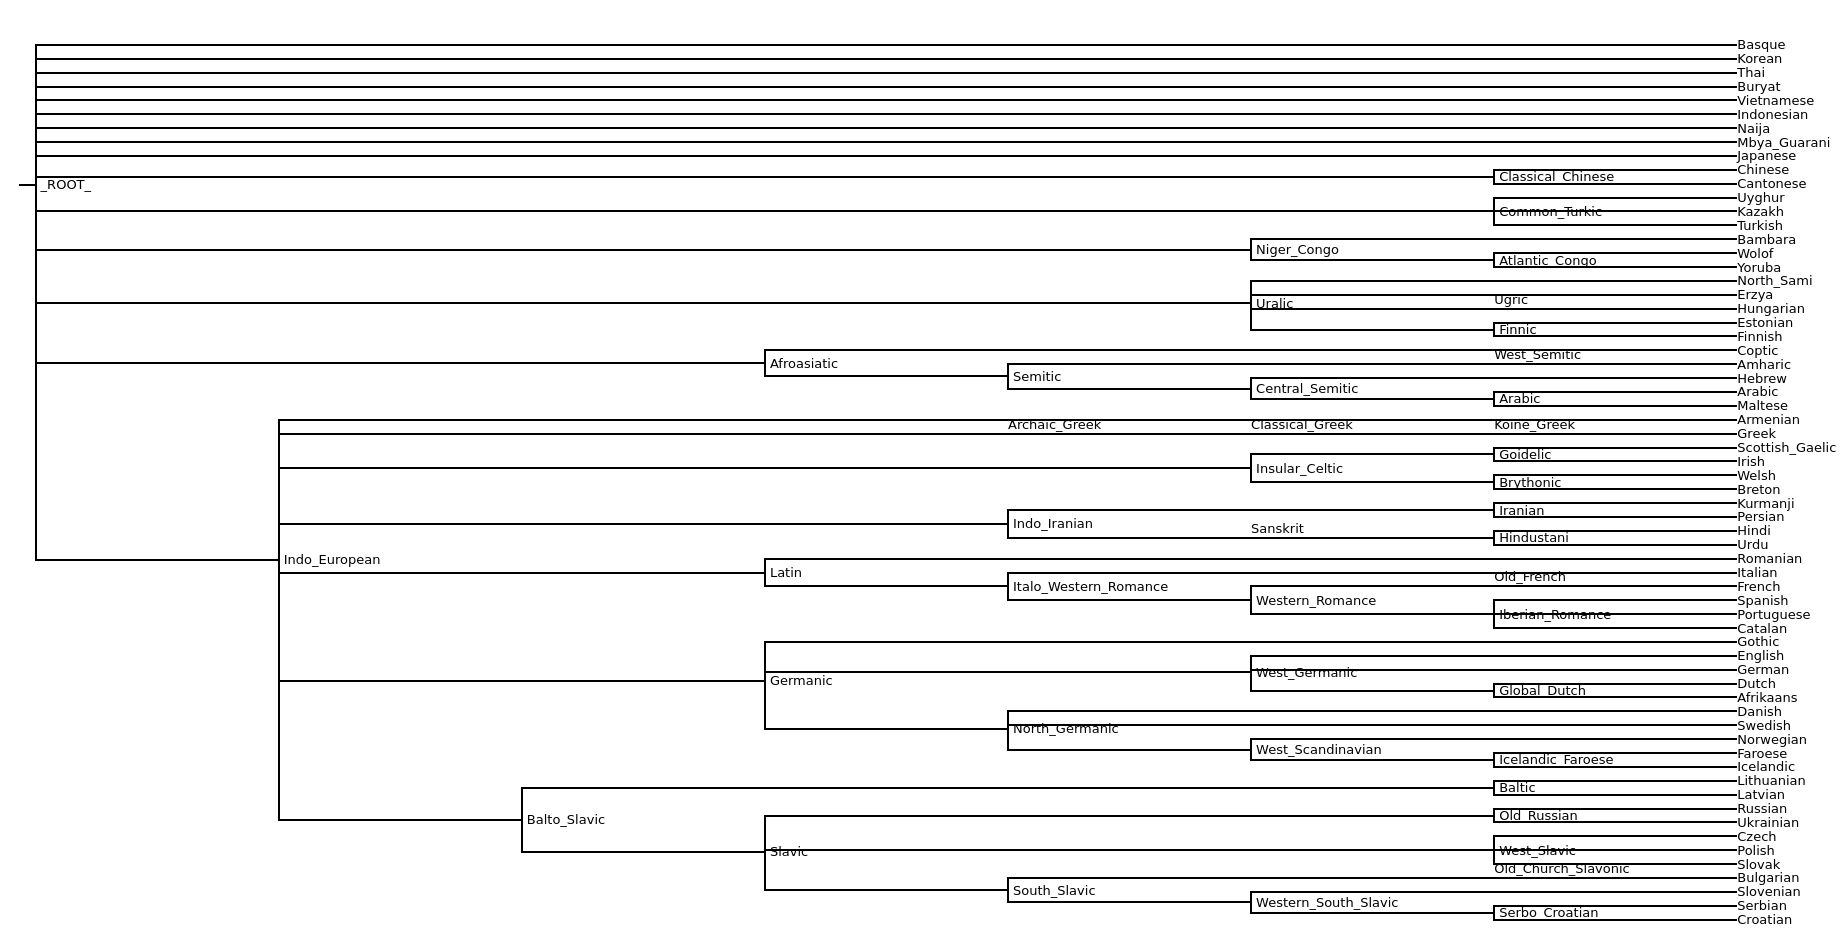
\includegraphics[width=1.3\textwidth]{../trees/tree.png}}
       \caption{Phylogenetic tree topology of the languages in our sample. Compare Figure~\ref{fig:tree-times} for a version indicating the time depth of different families.}
    \label{fig:tree}
\end{figure}


\begin{figure}
    \centering
	\rotatebox{270}{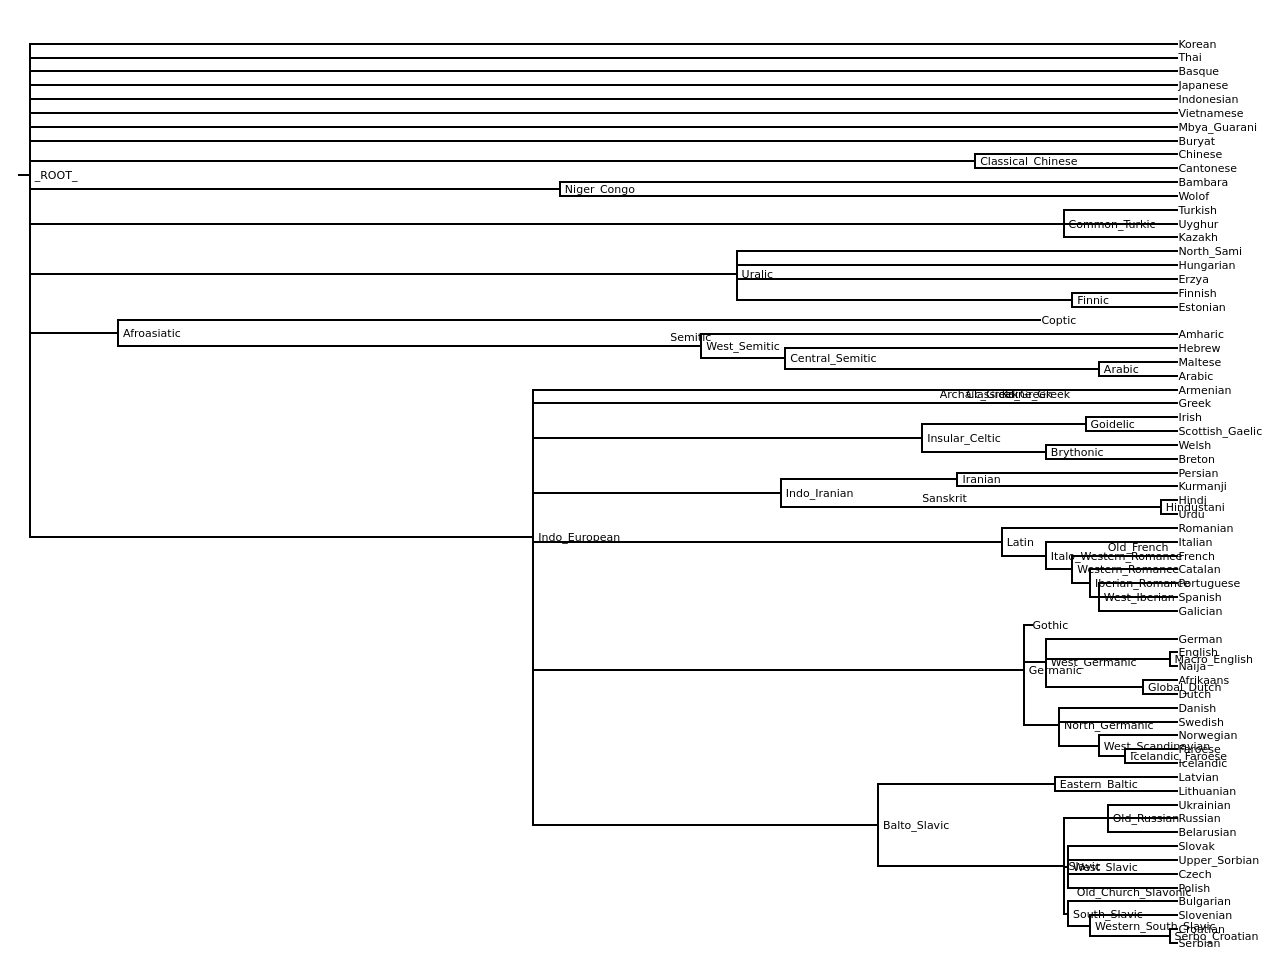
\includegraphics[width=1.3\textwidth]{../trees/tree-times.png}}
	\caption{Phylogenetic tree of the languages in our sample. The length of branches reflects distance in time. Compare Figure~\ref{fig:tree} for a version indicating the raw topology without time depths.}
    \label{fig:tree-times}
\end{figure}




\subsection{Dating Inner Nodes}
We labeled interior nodes for the time at which they split into descendants, using estimates based on historical evidence and the linguistic literature:


%Dates of split are not always strictly meaningful (e.g. for Romance).



\begin{longtable}{llp{10cm}lll}
Group & Split & Source or Rationale \\ \hline
Afroasiatic & 10,000 BC & \cite{diakonoff1998the} \\
Arabic & 1,100 AD & Calibration from \citep{holman2011automated} based on end of Arabic domination of Malta. \\
%Atlantic-Congo & 4,500 BC & \citet{holman2011automated} estimate an age of 6525 years.\\
Balto-Slavic & 1,400 BC & \citep{gray2003language} \\
	Brythonic & 500 AD & Migrations from Britain to Brittany \citep{holman2011automated}\\ % (Humphreys 1993:609. Breton language its present position and historical background, cited by 
Central-Semitic & 2,450 BC & \citep{kitchen2009bayesian}   \\
Common Turkic & 700AD & \cite[p. 49]{savelyev2020bayesian} estimate Common Turkic to have split around 474 AD. However, in their model, Old Turkic split off around 650 AD, earlier than the languages in our dataset, with uncertainty about the time of split of the remaining Common Turkic languages. It should predate the earliest documentation of Karluk Middle Turkic after 900AD. We thus put the divergence of the other Common Turkic languages at 700AD. \\
Eastern Baltic & 600 AD & Split between Latvian and Lithuanian \citep[p. 209]{novotna2011glottochronology}\\
Finnic & 800 AD & \cite[Section 4.1]{maurits2020best} \\
Germanic & 250AD & \cite{gray2003language} \\
Global Dutch & 1,600 AD & Dutch colony in South Africa \\
Goidelic & 950 AD & Migrations from Ireland to Scotland. \citet{holman2011automated}, citing \citet{jackson1951gaelic}, calibrates the divergence between Irish and Scottish Gaelic to 950 AD. \\
Hindustani & 1,800 AD & Standardization of Hindi and Urdu\\
Iberian Romance & 1,000 AD & Expansion of Christian kingdoms in Iberia, earliest Iberian Romance texts \\
Icelandic-Faroese & 1,400 AD & Sound shifts specific to Faroese\\
Indo-European & 5,300 BC & \citep{gray2003language} (excluding Hittite and Tocharian, for which we have no corpus data). \\
Indo-Iranian & 2,500 BC & \citep[p. 138]{parpola2013formation} \\ % Parpola 1999 suggests 2000 BC. The formation of the Aryan branch of Indo-European.
Insular Celtic & 900BC & \citep{gray2003language} estimate 900BC. \\ %Sound shift k$^w$ $>$ p in the Brythonic branch antedates attestation of name `Britain' in 325BC. \\ % Gray and Atkinson: 900BC. Language-tree divergence times support.. Rexova et al, Cladistic analysis
Iranian & 500 BC & \citep{gray2003language}. \\ % (Parpola 1999:200) suggests 1900BC based on archaeological evidence. \\ % Kurmanji, Persian. Parpola 1999 suggests 1900 BC.
Italo-Western-Romance & 500 AD & End of the Western Roman empire \citep{holman2011automated}.  \\
	Macro-English & 1900AD & In our dataset, this is the common ancestor of contemporary English and Naija (Nigerian Pidgin). \\
Niger-Congo & 5000BC & \citet{holman2011automated} estimate an age of 6227 years, but the family has to be older than Atlantic-Congo, which they estimate at 6525 years. We thus place Niger-Congo at 5000BC.\\
North-Germanic & 650 AD & Split of Old Norse into regional variants, such as assimilation of nasals to following stops in Western Norse in the 7th century \citep[p. 1856, 1859]{sandoy2017202}. Similarly \citep{holman2011automated} calibrates this to 900 AD. \\% (e.g. assimilation of nasals to following stop in Western Norse in the 7th century. Bandle 2005, Ch. XVII par. 202, The typological ...I Phonology Old East Nordic, p. 1856, 1859. \\
Semitic & 3,750 BC & \citep{kitchen2009bayesian} \\
Serbo-Croatian & 1,900 AD & Standardization of Serbian and Croatian\\
Slavic       & 700AD & \citep{gray2003language}. \citet[p. 209]{novotna2011glottochronology} date the split of East Slavic to the 6th century, \citep{holman2011automated} calibrates it to 550AD. \\
South-Slavic & 750 BC & Expansion of Slavic into Balkan. Postdates Slavic and antedates Old Church Slavonic (attested after 800AD) \\
Uralic & 3,000 BC & \citep[Section 4.7]{maurits2020best}, cf \citep[p. 144]{parpola2013formation} for references \\
West Iberian & 1,100AD & Independence of Portugal \\
West-Germanic & 500 AD & Migrations into Britain and southern central Europe\\
West-Scandinavian & 1,100 AD & Sound shifts specific to Norwegian\\
West-Semitic & 3,400 BC & \citep{kitchen2009bayesian}  \\
West-Slavic & 750 BC & Expansion of Slavic. \\ %\citet{holman2011automated} calibrates the split between Czech and Slovak at 1050AD.  \\ % , citing Fodor (1962:132),
Western Romance & 800 AD & Expansion of Christian kingdoms into Iberia \\
Western South Slavic & 1,000 AD & Antedates earliest Slovenian and Serbo-Croatian texts\\
\end{longtable}





\section{Details for Phylogenetic Models}



%We adopt the model of random walks on phylogenetic trees.
%We model the development of grammar and usage as an Ornstein-Uhlenbeck process (See SI Section X for results with a simpler Brownian motion model).
%According to the model of random walks on phylogenetic trees, whenever a (historical) language branches off into multiple successor languages, they independently develop according to this process.


%As the data for optimized grammars comes in the form of counts, we model the usage of a language $L$ as a latent variable $X_L$ that defines the log-odds that an optimized grammar has a subject-object position congruence of 1 (as opposed to 0).
%We model the state of the grammar as $Y_L$, the observed subject-object position congruence.
%$X_L$ and $Y_L$ together form the state $\xi_L \in \mathbb{R} \times [0,1]$  of the language.

%\subsection{Simple Brownian Motion Model}


%We model the instantaneous change of the state $\xi_t$ a language at a given time $t$ as a correlated Brownian motion in two dimensions:
%\begin{equation*}
%    d\xi_t = \Lambda dB_t
%\end{equation*}
%where $\Lambda \in \mathbb{R}^{2\times 2}$ is non-degenerate.

%\subsection{Model with Drift}

%(See below for likelihood results, showing poor fit of the simple Brownian model).


%\section{Details for Phylogenetic Models}



%We adopt the model of random walks on phylogenetic trees.
%We model the development of grammar and usage as an Ornstein-Uhlenbeck process (See SI Section X for results with a simpler Brownian motion model).
%According to the model of random walks on phylogenetic trees, whenever a (historical) language branches off into multiple successor languages, they independently develop according to this process.


%As the data for optimized grammars comes in the form of counts, we model the usage of a language $L$ as a latent variable $X_L$ that defines the log-odds that an optimized grammar has a subject-object position congruence of 1 (as opposed to 0).
%We model the state of the grammar as $Y_L$, the observed subject-object position congruence.
%$X_L$ and $Y_L$ together form the state $\xi_L \in \mathbb{R} \times [0,1]$  of the language.

%\subsection{Simple Brownian Motion Model}


%We model the instantaneous change of the state $\xi_t$ a language at a given time $t$ as a correlated Brownian motion in two dimensions:
%\begin{equation*}
%    d\xi_t = \Lambda dB_t
%\end{equation*}
%where $\Lambda \in \mathbb{R}^{2\times 2}$ is non-degenerate.

%\subsection{Model with Drift}


%This is expressed by the following stochastic differential equation, known as the Ornstein-Uhlenbeck process:
%We model the instantaneous change of the state $\xi_t$ a language at a given time $t$ as a combination of drift and Brownian motion:
%\begin{equation*}
%    d\xi_t = -A(\xi_t-\mu) + \Lambda dB_t
%\end{equation*}
%where $A, \Lambda \in \mathbb{R}^{2\times 2}$, all eigenvalues of $A$ have positive real part, and $\Lambda$ has full rank.


%The matrix $A$ encodes the direction of drift.
%$A_{1,2}$ encodes the extent to which drift of $X_t$ and $Y_t$ is correlated:
%$A_{1,2} > 0$ means that languages drift in such a way that $X_L, Y_L$ are positively correlated (coadaptation); $A_{0,0} = 0$ means that languages do not drift towards a correlation (See Si Section X for an alternative formulation in terms of correlated Brownian motion).


%We model the instantaneous change of the state $\xi_t \in \mathbb{R}^2$ of a language at a given time $t$ as a combination of drift and Brownian motion, formalized by the following stochastic differential equation defining the Ornstein-Uhlenbeck process \citep[p. 109, eq. 4.4.42]{gardiner1983handbook}:
%\begin{equation*}
%    d\xi_t = -\Gamma \cdot (\xi_t-\mu) dt + \Lambda \cdot dB_t
%\end{equation*}
%where $\mu \in \mathbb{R}^2$, $\Gamma, \Lambda \in \mathbb{R}^{2\times 2}$, the real part of each eigenvalue of $\Gamma$ is positive, and $\Lambda$ has full rank (so that $\Lambda\Lambda^T$ is positive definite).
%is positive definite, and $\Lambda$ is diagonal with positive entries (see SI Section for results with non-diagonal $\Lambda$).


%The matrix $A$ encodes the direction of drift.
%$A_{1,2}$ encodes the extent to which drift of $X_t$ and $Y_t$ is correlated:
%$A_{1,2} > 0$ means that languages drift in such a way that $X_L, Y_L$ are positively correlated (coadaptation); $A_{0,0} = 0$ means that languages do not drift towards a correlation (See Si Section X for an alternative formulation in terms of correlated Brownian motion).


%We model the instantaneous change of the state $\xi_t \in \mathbb{R}^2$ of a language at a given time $t$ as a combination of drift and Brownian motion, formalized by the following stochastic differential equation defining the Ornstein-Uhlenbeck process \citep[p. 109, eq. 4.4.42]{gardiner1983handbook}:
%\begin{equation*}
 %   d\xi_t = -\Gamma \cdot (\xi_t-\mu) dt + \Lambda \cdot dB_t
%\end{equation*}
%where $\mu \in \mathbb{R}^2$, $\Gamma, \Lambda \in \mathbb{R}^{2\times 2}$, the real part of each eigenvalue of $\Gamma$ is positive, and $\Lambda$ has full rank (so that $\Lambda\Lambda^T$ is positive definite).
%is positive definite, and $\Lambda$ is diagonal with positive entries (see SI Section for results with non-diagonal $\Lambda$).


%The matrix $A$ encodes the direction of drift.
%$A_{1,2}$ encodes the extent to which drift of $X_t$ and $Y_t$ is correlated:
%$A_{1,2} > 0$ means that languages drift in such a way that $X_L, Y_L$ are positively correlated (coadaptation); $A_{0,0} = 0$ means that languages do not drift towards a correlation (See Si Section X for an alternative formulation in terms of correlated Brownian motion).

%, for comparison with a simple Brownian motion model, and for comparison with non-diagonal $\Gamma$.
%We adopt the model of Brownian motion on phylogenetic trees.
%As the data for optimized grammars comes in the form of counts, we model the usage of a language $L$ as a latent variable $X_L$ that defines the log-odds that an optimized grammar has a subject-object position congruence of 1 (as opposed to 0).
%We model the state of the grammar as $Y_L$, the observed subject-object position congruence.
%$X_L$ and $Y_L$ together form the state $\xi_L \in \mathbb{R} \times [0,1]$  of the language.
%We model the instantaneous change of the state $\xi_t$ a language at a given time $t$ as Brownian motion:
%\begin{equation*}
%    d\xi_t = \Lambda dB_t
%\end{equation*}
%where $\Lambda \in \mathbb{R}^{2\times 2}$.
%$\Lambda_{1,2}$ encodes the extent to which drift of $X_t$ and $Y_t$ is correlated:
%$A_{1,2} > 0$ means that languages drift in such a way that $X_L, Y_L$ are positively correlated (coadaptation); $A_{0,0} = 0$ means that movement in both directions is not correlated.

%The matrix $\Sigma := \Lambda\Lambda^T$ indicates the variance-covariance structure of the instantaneous changes at any time $t$.
%The main quantity of interest is the correlation between changes in the two dimensions, which is given by
%\begin{equation}
%R := \frac{\Sigma_{1,2}}{\sqrt{\Sigma_{1,1}\Sigma_{2,2}}}
%\end{equation}
%A positive value indicates that changes in both directions are positively correlated.

\subsection{Calculating the Likelihood}
For completeness, we describe how to calculate the likelihood of a multidimensional Ornstein-Uhlenbeck model on phylogenetic trees \citep{felsenstein1988phylogenies,hansen1997stabilizing, blackwell2003bayesian}.

As described in the Methods section, it is described by the following stochastic differential equation for the instantaneous change of the state $\xi_{L,t}$ of a language $L$ at a given time $t$:
\begin{equation}\label{eq:sde}
    \operatorname{d}\xi_{L,t} = \Gamma \cdot (\xi_{L,t}-\mu) \operatorname{d}t + \Lambda \operatorname{d}B_t
\end{equation}
where $\mu \in \mathbb{R}^2$,  $\Gamma, \Lambda \in \mathbb{R}^{2\times 2}$ are non-degenerate matrices, and $B_t$ is Brownian motion in two dimensions.

In our model, $\Gamma$ is diagonal with positive entries; we found no improved model fit when taking more general choices for $\Gamma$.

The conditional distribution of a future observation at time $t+\Delta$ given an earlier one at time $t$ is given by the following equation \citep[Theorem 3.3]{schach1971weak}, \citep{gardiner1983handbook}, \citep[p. 156, eq. 6.124]{risken1989fokker}:
\begin{equation}
\xi_{L,t+\Delta} | \xi_{L,t} \sim N\left(\mu + e^{-\Delta \Gamma} (\xi_{L,t}-\mu),\ \Omega - e^{-\Delta \Gamma} \Omega e^{-\Delta \Gamma^T}\right)
\end{equation}
where the matrix $\Omega \in \mathbb{R}^{2\times 2}$ is obtained as the solution of the equation \citep[p. 110, eq. 4.4.51]{gardiner1983handbook} \citep[p. 156, eq. 6.126]{risken1989fokker}:
\begin{equation}
    \Gamma\Omega+\Omega\Gamma^T = \Lambda \Lambda^T
\end{equation}
Setting $\Sigma := \Lambda\Lambda^T$, this can be solved as follows:\footnote{More generally, if $\Gamma$ is not diagonal:
\begin{equation}\label{eq:sigma-omega}
\left(\begin{matrix} \Omega_{11} \\ \Omega_{12} \\ \Omega_{22} \end{matrix}\right)=    \left(\begin{matrix}
    2\Gamma_{11} & 2\Gamma_{12} & 0 \\
    \Gamma_{21} & \Gamma_{11}+\Gamma_{22} & \Gamma_{12} \\
    0 & 2\Gamma_{21} & 2\Gamma_{22}
    \end{matrix}\right)^{-1}  \left(\begin{matrix} \Sigma_{11} \\ \Sigma_{12} \\ \Sigma_{22} \end{matrix}\right)
\end{equation}
}
\begin{equation}\label{eq:sigma-omega}
\left(\begin{matrix} \Omega_{11} \\ \Omega_{12} \\ \Omega_{22} \end{matrix}\right)=   \left(\begin{matrix} \frac{\Sigma_{11}}{2\Gamma_{11}}  \\ \frac{\Sigma_{12}}{\Gamma_{11}+\Gamma_{22}} \\ \frac{\Sigma_{22}}{2\Gamma_{22}} \end{matrix}\right)
\end{equation}
One can compute the stationary distribution that solves the differential equation as follows.
The stationary distribution of an individual observation is
\begin{equation}\label{eq:ornuhl-var}
\xi_{t} \sim N\left(\mu, \Omega \right)
\end{equation}
The stationary cross-covariance between the states of two languages $L_1, L_2$, possibly on different branches of the phylogenetic tree, is given by
\begin{equation}\label{eq:ornuhl-covar}
Cov(\xi_{L_1}, \xi_{L_2}) = e^{-\Delta_1 \Gamma} \Omega e^{-\Delta_2 \Gamma^T}
\end{equation}
where $\Delta_1, \Delta_2$ are the times of evolution from their last common ancestor to $L_1$ and $L_2$, respectively.
\footnote{This can be shown as follows:
If $\xi_A$ is the last common ancestor, then (we set $\mu=0$ without loss of generality, as it does not affect the covariance):
\begin{align*}
Cov(\xi_{L_1}, \xi_{L_2}) &= \mathbb{E} \left[\xi_{L_1} \xi_{L_2}^T\right] - \mathbb{E}\xi_{L_1} \mathbb{E}\xi_{L_2}^T   &= \mathbb{E}\left[\mathbb{E} \left[\xi_{L_1} \xi_{L_2}^T | \xi_A\right]\right] - 0 \cdot 0  &= \mathbb{E}\left[\mathbb{E} \left[\xi_{L_1}|\xi_A\right] \mathbb{E} \left[\xi_{L_2}^T | \xi_A\right]\right]  
 &= \mathbb{E}\left[   e^{-\Delta_1\Gamma} \xi_A    \xi_A^T e^{-\Delta_2\Gamma^T} \right]  \\
 &= e^{-\Delta_1\Gamma} \Omega e^{-\Delta_2\Gamma^T}   \\
\end{align*}}
If $L_1, L_2$ do not share a common ancestor (the root in Figure~\ref{fig:tree} does not count as an ancestor), the covariance is zero.\footnote{As $\lim_{\Delta \rightarrow \infty} e^{-\Delta B} = 0$, this is practically equivalent to assuming a very large time-depth of the last common ancestor, which would be the case under the assumption of macrofamilies with very large time depth.}



Since any Ornstein-Uhlenbeck process is Gaussian \citep{schach1971weak}, the joint distribution of any set of observations $\xi_{L, t}$ is determined by (\ref{eq:ornuhl-var}-\ref{eq:ornuhl-covar}).

\subsection{Implementation}\label{sec:prior-lkj}

We defined the following priors on the parameters.
We parameterized $\Lambda$ as $D U$, where $U$ is a lower-diagonal matrix, and $D$ is a diagonal matrix.
This is equivalent to modeling $\Sigma := \Lambda\Lambda^T$ as the combination of a correlation matrix and a vector of standard deviations \citep{barnard2000modeling}.
Analogously, we parameterized $\Gamma := E E^T$, where $E$ is also a diagonal matrix.

To define a prior over $\Lambda$, we modeled $U$ as the lower Cholesky factor of a correlation matrix subject to an LKJ(1) prior (\citet{lewandowski2009generating}, i.e., the uniform distribution over $2\times 2$-correlation matrices).
We placed a standard normal prior $N(0,1)$ on the entries of $\mu$ and on the non-zero entries of $D, E$.

We rescaled times so that 1000 years corresponded to one unit, and rescaled position congruences to range from -1 to 1 (instead of 0 to 1).

We implemented the models in Stan~\citep{carpenter2017stan} and obtained posterior samples using the No-U-Turn sampler.
We ran four chains with 2000 iterations each, of which the first 1000 were discarded as warmup samples.

We computed marginal likelihoods using Stepping Stone Sampling \citep{xie2011improving} with $K=10$ stones.
The fact that $Y_L$ is a latent variable complicates computation of the likelihood; we approximated this by fixing $Y_L$ to the log-odds of the observed empirical counts, adding $1$ to each category to smooth out cases where $Y_L =0,1$.
We verified stability of the estimates by running the procedure ten times for each model, and averaging the obtained marginal likelihoods.

%\subsection{Robustness to Priors}
%
%with of the normal priors
%
%TODO
%
%describe priors
%
%- change width of the normal priors
%
%- change prior for $\Omega_{12}$ to a truncated normal, shrinking towards zero correlation (biasing towards the null hypothesis of uncorrelated change)
%
%In Table we show estimated stationary correlations and marginal log-likelihoods across these priors.
%
%\begin{table}
%\begin{tabular}{llllll}
%	...
%\end{tabular}
%	\caption{Robustness to prior choices, for the parameterization described in Section~\ref{sec:prior-lkj}.}
%\end{table}
%
%
%

%describe priors
%
%In Table we show estimated stationary correlations and marginal log-likelihoods across these priors.
%
%\begin{table}
%\begin{tabular}{llllll}
%	...
%\end{tabular}
%	\caption{Robustness to prior choices}
%\end{table}
%

\subsection{Alternative Parameterizations}\label{sec:alt-param}
The parameterization described above places separately priors on the drift ($\Gamma$) and diffusion ($\Sigma = \Lambda\Lambda^T$) components of the Ornstein-Uhlenbeck process.
While such a parameterization closely mirrors the parameters occurring in Equation~\ref{eq:sde}, it may suffer from slow convergence of Markov chains or diverging transitions when data is limited, as drift and diffusion components are not always individually identifiable (even when the correlation component of $\Sigma$ -- the key parameter for evaluating the coadaptation hypothesis --  is identifiable).
We therefore also considered another parameterization that eliminates such problems by intstead placing a prior on $\Omega$ and $\Gamma$, and deriving $\Sigma$ from those.
We use Gaussian priors for the variance components of $\Omega$ and the diagonal entries of $\Gamma$, and a uniform prior for the correlation component of $\Omega$:
\begin{align*}
\Omega_{11}, \Omega_{22} & \sim HalfNormal(0,1) \\
\Omega_{12} & \sim Uniform(-1,1) \sqrt{\Omega_{11} \Omega_{22}} \\
\Gamma_{11}, \Gamma_{2,2} & \sim HalfNormal(0,1) \\
\end{align*}
Due to Equation~\ref{eq:sigma-omega}, $\Sigma$ is then obtained as
\begin{align*}
	\Sigma_{11} &= 2 \Gamma_{11} \Omega_{11}  \\
	\Sigma_{12} &= (\Gamma_{11} + \Gamma_{22}) \Omega_{12} \\
	\Sigma_{22} &= 2 \Gamma_{22} \Omega_{22}
\end{align*}
With this prior, the correlation of the two dimensions in the stationary distribution was estimated as $R=0.77$ (95\% CrI $[0.35, 0.97]$) for the full dataset, and $R = 0.83$ (95\% CrI $[0.43, 0.99]$) excluding the Indo-European languages.
The Bayes factor in favor of the full model with a nonzero correlation, compared to a lesioned model with zero correlation, was 117. %change/ornuhl-binom-reparam/noLatents_logodds_approx_Reparam/marginal_likelihood

A possible concern with both the LKJ prior in Section~\ref{sec:prior-lkj} and the uniform prior described here for $\Omega_{12}$ is that they do not regularize towards small correlations.
However, the posterior for the correlation of the two dimensions in the stationary distribution was estimated very similarly ($R = 0.81$, $95\%$ CrI $[0.43,  0.99]$) when using a prior that explicitly regularizes towards small correlations:
\begin{equation}
	\Omega_{12} \sim Normal(0,1)_{Truncated\ to\ [-1,1]} \sqrt{\Omega_{11} \Omega_{22}}
\end{equation}


We further considered a version of the model where we modeled the state of usage as the average optimized subject-object position congruence (and not the log-odds of observing either result in an individual optimized grammar).
In this model, the correlation of the two dimensions in the stationary distribution was estimated as $R = 0.77$ ($95\%$ CrI $[0.45, 0.93]$, $P(R \leq 0) = 0.00075$). % change/ornuhl-binom_LINEAR/noLatents_Reparam_LINEAR/fits/correlation_omega.txt
%and (TODO, TODO, TODO) excluding Indo-European.
The Bayes factor in favor of the full model with a nonzero correlation was 66.
We also considered a version where attested and optimized subject-object congruence were subject to observation noise, assuming a $HalfNormal(0,1)$ prior for both variance parameters.
While marginal likelihood did not support increasing model complexity in this way (Bayes factor $8.3$ in favor of the model without observation noise), parameter fit was in agreement with the other models: The correlation of the two dimensions in the stationary distribution was estimated as $R = 0.80$ ($95\%$ CrI $[0.13, 0.99]$, $P(R \leq 0) = 0.017$). % for the full dataset % change/ornuhl-binom_LINEAR/noLatents_Reparam_noise_LINEAR/fits/correlation_omega.txt
%and (TODO, TODO, TODO) excluding Indo-European.

%
%\paragraph{Robustness to Priors}
%describe priors
%
%- change width of the normal priors
%
%- change prior for $\Omega_{12}$ to a truncated normal, shrinking towards zero correlation (biasing towards the null hypothesis of uncorrelated change)
%
%In Table we show estimated stationary correlations and marginal log-likelihoods across these priors.
%
%\begin{table}
%\begin{tabular}{llllll}
%	...
%\end{tabular}
%	\caption{Robustness to prior choices, for the parameterization described in Section~\ref{sec:alt-param}.}
%\end{table}
%
%
%

\subsection{Correlation Component of $\Sigma$}\label{sec:instant-corr}
In the main analysis, we reported the correlation between the two dimensions in the stationary distribution $\Omega$.
In some of the analyses in the SI, there are multiple stationary distributions (depending on geography, case marking, or categorical order classes, see Sections 5--7).
In these cases, we therefore report correlation for the instantaneous changes at any point in time:
The matrix $\Sigma := \Lambda\Lambda^T$ indicates the variance-covariance structure of the instantaneous changes at any time $t$ \citep{felsenstein1973maximum, freckleton2012fast}.
The main quantity of interest is the correlation between changes in the two dimensions \citep[cf.][]{felsenstein1973maximum,freckleton2012fast}, which is given by
\begin{equation}
R_\Sigma := \frac{\Sigma_{1,2}}{\sqrt{\Sigma_{1,1}\Sigma_{2,2}}}
\end{equation}
A positive value indicates that changes in both directions are positively correlated.
%We show the posterior of $R_\Sigma$ for the main analysis in Figure~\ref{fig:corr-main}.
%
%\begin{figure}
%    \centering
%	\begin{tabular}{cccc}
%    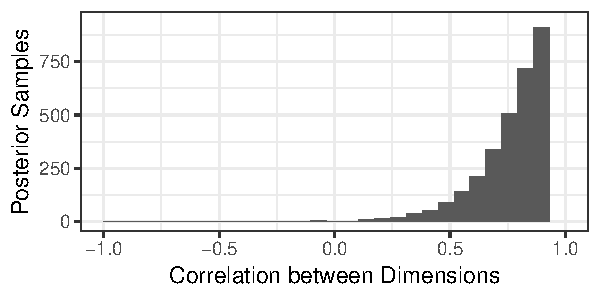
\includegraphics[width=0.5\textwidth]{../change/ornuhl-binom/noLatents/fits/corr_sigma.pdf} \\
%	\end{tabular}
%    \caption{Posterior of the correlation component $R_\Sigma$ (see Section~\ref{sec:instant-corr}) in the main analysis.}
%    \label{fig:corr-main}
%\end{figure}
%


%\paragraph{Computing Likelihood for Brownian Motion Model}

%We impose an LKJ prior on the correlation matrix of $A$, a student $t$ prior on the variance components of $A$ and $\Lambda$, a ... prior on the two components of $\Lambda$.

%\paragraph{Computing Likelihood for Ornstein-Uhlenbeck Model}

\section{Comparison with Simple Brownian Model}

The simple Brownian model leaves out the drift term, leading to the stochastic differential equation:
\begin{equation*}
    \operatorname{d}\xi_t = \Lambda \operatorname{d}B_t
\end{equation*}
This is known as the Independent Contrasts model \citep{felsenstein1973maximum, freckleton2012fast}.

Brownian motion differs from the Ornstein-Uhlenbeck process in that it does not have a long-term stationary solution.
Instead, trajectories $\xi_t$ tend to move arbitrarily far away from the origin over time $t$.
This is clearly unrealistic in our setting, as subject-object position congruence is bounded between 0 and 1.
As there is no stationary solution, there is no straightforward way to jointly apply the model to data from languages that do not share a common ancestor.
For modelling purposes, we assumed that all families had a common ancestor at some large time $T_0$ in the past.
This modelling assumption corresponds to the assumption of macro-families of very large time-depth.
We considered $T_0$ to be 20,000 BC, 50,000 BC, and 100,000 BC, and measured the instantaneous correlation of changes $R$ for each fit.
To evaluate model fit, we compared marginal likelihood of the Brownian model with the Ornstein-Uhlenbeck model.
Note that an assumption of a specific time depth is not necessary for the Ornstein-Uhlenbeck model, as unrelated languages can be modeled as draws from the stationary distribution for that model.

\paragraph{Results}
Across different choices of $T_0$, the Brownian model strongly supports a positive correlation $R$, very similar to the Ornstein-Uhlenbeck analysis; the posterior probability of $R\leq 0$ is $0.00025$ at $T_0=-100,000$, $0.00025$ at $T_0 = -50,000$, and $0$ at $T_0 = -20,000$. %change/brownian-binom/fits
When excluding the Indo-European phylum, this probability is $0.0028$ at $T_0=-100,000$, $0.0015$ at $T_0=-50,000$, and $0.0005$ at $T_0 = -20,000$.
However, model fit as measured by marginal likelihood is much weaker than in the Ornstein-Uhlenbeck model, across choices of $T_0$ (Table~\ref{tab:marg-brown}), corresponding to a Bayes factor of about $10^{55}$ in favor of the Ornstein-Uhlenbeck model for the full dataset and $10^{15}$ when excluding Indo-European.

\begin{table}
	\begin{center}
	\textbf{Full Dataset}
	
	\begin{tabular}{llllllll}
	% change/brownian-binom/logodds-approx/marginal_likelihood$ more results.txt
	Model & Log-Likelihood \\ \hline
	Ornstein-Uhlenbeck & -32 \\
	Ornstein-Uhlenbeck (diagonal $\Sigma$) & -38 \\
	Brownian ($T_0 = -100,000$) & -190 \\
	Brownian ($T_0 = -50,000$) & -188 \\
	Brownian ($T_0 = -20,000$) & -170
\end{tabular}
	\end{center}
	
		\begin{center}
\textbf{Indo-European Excluded}
	
	\begin{tabular}{llllllll}
	% change/brownian-binom/logodds-approx/marginal_likelihood$ more results.txt
	Model & Log-Likelihood \\ \hline
	Ornstein-Uhlenbeck & -29 \\
	Ornstein-Uhlenbeck (diagonal $\Sigma$) & -33 \\
	Brownian ($T_0 = -100,000$) & -79 \\
	Brownian ($T_0 = -50,000$) & -71 \\
	Brownian ($T_0 = -20,000$) & -64
\end{tabular}
	\end{center}
	\caption{Marginal log-likelihoods for Ornstein-Uhlenbeck and simple Brownian models. Values closer to $0$ indicate better model fit. We ran the Brownian model at different time depths, because it does not have a stationary distribution.}
	\label{tab:marg-brown}
\end{table}



\section{Accounting for Areal Convergence}
The model of random walks on phylogenetic trees assume that languages evolve independently once they have split~\citep[e.g.][]{dunn-evolved-2011, maurits2014tracing}.
However, linguistic evolution can include borrowing between geographically neighboring languages \citep[e.g.][]{dryer1989large, bisang1996areal, heine2003on, aikhenvald2007grammars,  kalyan2019problems}.

Here, we provide evidence that our conclusions continue to hold when explicitly modelling convergence in linguistic areas, geographic regions in which languages tend to show convergent evolution due to borrowing  \citep[e.g.][]{campbell1986meso, nichols1992linguistic, haspelmath2001the, gijn2017linguistic}.

We modeled linguistic areas as latent variables defining time- and location-dependent values $\mu(x,t)$ (where $x$ is a point on the surface of the earth and $t$ is a point in time) that languages at time $t$ and place $x$ drift towards.
These values are inferred from the data together with the other parameters of the Ornstein-Uhlenbeck process.
By placing a suitable Gaussian process prior on $\mu(x,t)$, we encourage parameters that smoothly vary over space and time, reflecting the idea that areal convergence between languages depends on their geographic distance.
This approach is related to the model described by \citep{nuismer2015predicting}, who propose to model convergence between species by assuming correlations between the means $\mu$ of different species.
For other approaches to model interactions between species from the bioinformatics literature, see \citet{manceau2016a,drury2016estimating, bartoszek2017using, drury2018an}.


\paragraph{Model}
We model the grammar and usage components of $\mu$ as depending on the language's geographic position and the time a language was spoken.
This models the impact of linguistic areas, and allows this impact to change over time.

We assume that a language $L$ observed at time $t+\Delta$ (e.g. Modern English) developed from a prior state at time $t$ (e.g., Old English) during time $[t, t+\Delta]$ according to the Ornstein-Uhlenbeck SDE
\begin{equation}
    \operatorname{d}\xi_{L,t} = \Gamma \cdot (\xi_{L,t}-\mu_L) \operatorname{d}t + \Lambda \operatorname{d}B_t
\end{equation}
where $\mu_L$ is defined by the temporal and geographical location of the language $L$.


We placed a Gaussian process prior with a Laplace kernel on $\mu$.
That is, the covariance between $\mu$ at points $x, y$ on the surface of the earth at times $T_1, T_2$ is taken to be
\begin{equation}\label{eq:kernel}
    Cov(\mu_x, \mu_y) = \alpha \cdot \exp\left(-\frac{1}{\rho^2_1} d(x,y) - \frac{1}{\rho_2^2} |T_1-T_2|\right)
\end{equation}
where $d(x,y)$ is the great circle (geodesic) distance between points $x, y$, and $\alpha, \rho>0$ are hyperparameters.
The Laplace kernel is positive-definite with the great-circle distance $d(\cdot, \cdot)$ \citep{feragen2015geodesic} and thus provides a valid covariance for this distance; many other popular kernels like the RBF kernel are not valid for this distance \citep{feragen2015geodesic}.
This prior favors values of $\mu_L$ that vary smoothly over space and time, encoding the idea of linguistic areas.
We placed Gaussian priors with mean $0$ and variance $1$, truncated to positive values, on the hyperparameters $\alpha, \frac{1}{\rho^2}$ of the kernel~(\ref{eq:kernel}).


We extracted locations of languages from the World Atlas of Linguistic Structures \citep{haspelmath2005the}.
For ancestors, we recursively defined their location as the mean of the locations of their immediate children.


%As $\mu$ now varies with time, the resulting process is not Gauss-Markov any more \citep{schach1971weak}, and thus the likelihood cannot be represented with a single covariance matrix any more. We thus perform inference by explicitly modelling $\xi_L$ for all inner nodes $L$ of the phylogenetic tree.



\paragraph{Results}
We plot the posterior of the correlation component of $\Sigma$ (see Section~\ref{sec:instant-corr}) in Figure~\ref{fig:posterior-area-time}.
The posterior probability that the correlation is $\leq 0$ is estimated to be 0.00125.
In the stationary distribution, the two components are correlated at $R = 0.59$ (95\% credible interval $[0.25, 0.89]$); this quantity was estimated at $R = 0.66$ (95\% credible interval $[0.11, 0.94]$) when excluding Indo-European.
This confirms that coadaptation is found even when explicitly modeling convergence between neighboring languages.


\begin{figure}
	\begin{center}
    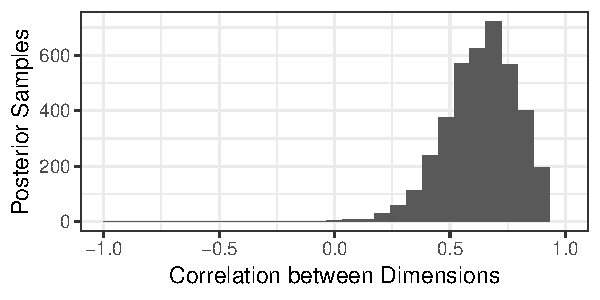
\includegraphics[width=0.45\textwidth]{../change/ornuhl-binom-geo-time/fits/corr_sigma.pdf}
	\end{center}
	\caption{Posterior of the correlation component of $\Sigma$ (see Section~\ref{sec:instant-corr}) when accounting for areal convergence.}\label{fig:posterior-area-time}
\end{figure}


%In Table, we show all models together with the logarithm of the estimated marginal likelihood of the data.
%Higher marginal likelihood indicates better model fit.


%Conditions:
%- $\Gamma$ has positive eigenvalues
%- $\Gamma\Omega+\Omega\Gamma^T$ is a covariance matrix
%- $\Omega$ is a covariance matrix
%Things to visualize
%- stationary distribution
%- instantaneous distribution over change directions


% https://courses.helsinki.fi/sites/default/files/course-material/4523939/Freckleton02.pdf


\section{Subject-Object Position Congruence and Categorical Classification of Basic Word Order}\label{sec:categorical}


\begin{figure}
    \centering
    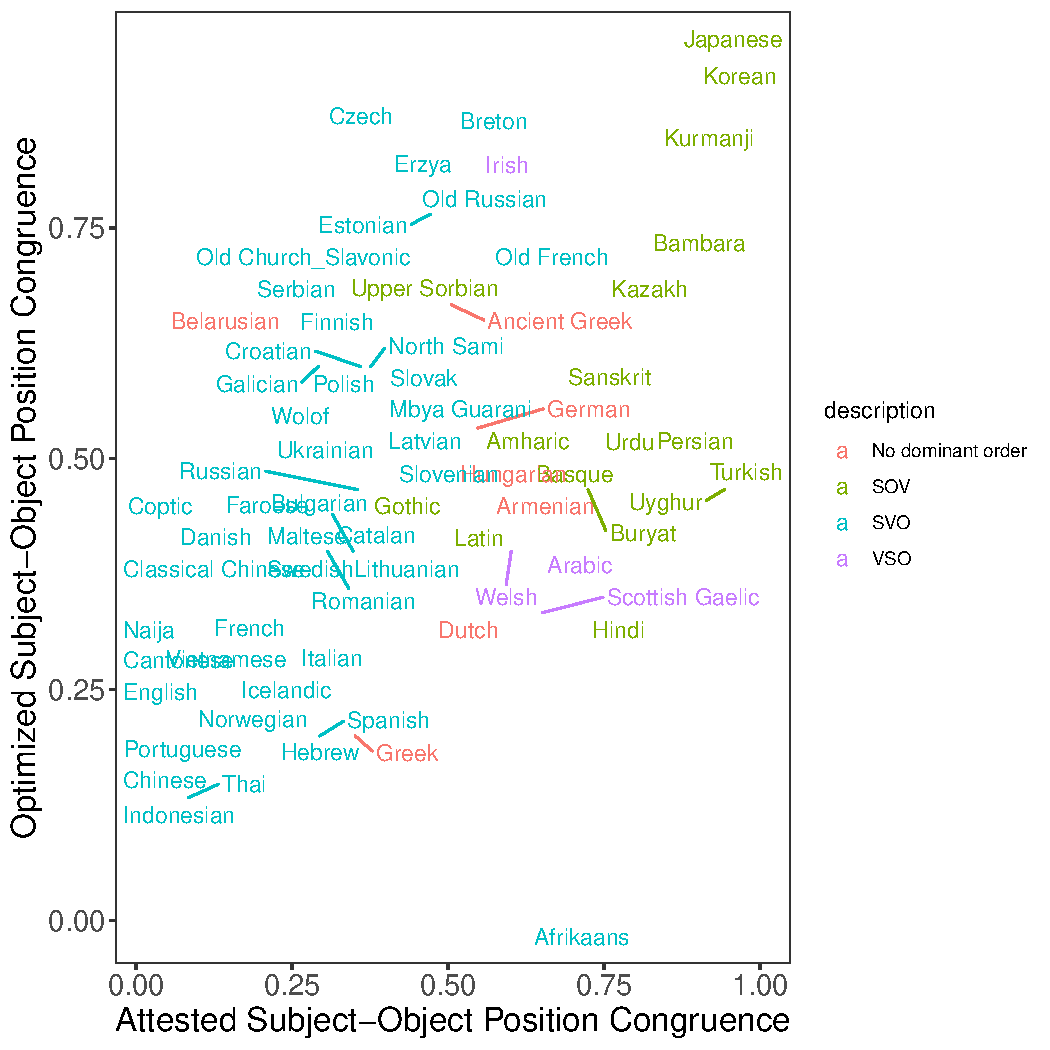
\includegraphics[width=0.6\textwidth]{../analysis/categorical_order/figures/by_categorical_order.pdf}
	\caption{Basic word orders as labeled in the World Atlas of Language Structures \citep{wals-81}, supplemented with data from other sources (see Section~\ref{sec:categorical}).}
    \label{fig:categorical-basic-order}
\end{figure}



The notion of subject-object position congruence addresses a key limitation of the standard classification of languages into basic word order categories by accounting for the well-documented differences in degrees of word order flexibilities in languages that are conventionally assigned the same basic word order \citep{steele1978word}.
Here, we compare subject-object position congruence to basic word order as classified in the typological literature.


In Figure~\ref{fig:categorical-basic-order}, we show attested and optimized subject-object position congruence, together with categorical basic word order labels from the World Atlas of Linguistic Structure \citep{wals-81}, supplemented with data from other sources where it had no data (primarily \citep{gell-mann-origin-2011}, see Table~\ref{tab:categorical}).
First, we see that attested subject-object position congruence largely determines whether a language is labeled SVO or SOV/VSO.
A few language with medium subject-object position congruence are labeled as `No dominant order'.

Optimized subject-object position congruence remains predictive of attested subject-object order even within the categories SVO ($R = 0.52, p = 0.0002$) and SOV ($R=0.45, p = 0.07$).
This suggests that the coadaptation theory makes predictions about word order beyond categorical notions of basic word order.

Next, we describe a version of the phylogenetic analysis controlling for catgeorical order.

\subsection{Phylogenetic Analysis}\label{sec:categorical}


\paragraph{Model}

We constructed a version of the phylogenetic analysis where the drift parameters $\mu, \Gamma$ depend on the categorical order of the language $L$:
\begin{equation*}
    \operatorname{d}\xi_{L,t} = \Gamma_{C(L)} \cdot (\xi_{L,t}-\mu_{C(L)}) \operatorname{d}t + \Lambda \operatorname{d}B_t
\end{equation*}
where $C(L)$ is the categorical order assigned to the language.

\paragraph{Labeling Categorical Basic Word Order}
This model requires labeling all nodes on the phylogenetic tree for categorical word orders.
For documented languages, we based the annotation on \citet{wals-81}.
In those languages where no annotation was available, we drew on \citep{gell-mann-origin-2011}, supplemented with language-specific literature.
In some cases, both `No dominant order' and one of SVO/SOV are plausible labels. In these cases, we opted for SOV/SVO, as we expect this to \emph{increase} the amount of variance that categorical order classes can explain, introducing at most a \emph{conservative} bias in estimating coadaptation.
We obtained the labels listed in Table~\ref{tab:categorical} for documented languages, and in Table~\ref{tab:interior} for non-attested nodes in the phylogenetic tree.

\begin{table}
\begin{tabular}{llp{0.5\textwidth}lll}
\hline
	Language & Label & Rationale \\ \hline
Afrikaans & SVO & \citet{gell-mann-origin-2011}\\
Archaic Greek & No dominant order & \citet{gell-mann-origin-2011} entry for `Classical Greek'\\
Classical Chinese & SVO &  \citet{pulleyblank1995outline}, unambiguously confirmed by UD data.\\
Classical Greek & No dominant order & \citet{gell-mann-origin-2011} entry for `Classical Greek'. Also labeled like this in \citet{wals-81}, Figure 1\\
Faroese & SVO & \citet{gell-mann-origin-2011}\\
Galician & SVO & \citet{gell-mann-origin-2011}\\
Gothic & SOV & \citet{gell-mann-origin-2011}\\
Kazakh & SOV & \citet{gell-mann-origin-2011}\\
Koine Greek & No dominant order & \citet{gell-mann-origin-2011} entry for `Classical Greek'\\
Latin & SOV & \citet{gell-mann-origin-2011}\\
Maltese & SVO & \citet{gell-mann-origin-2011}\\
Naija & SVO & Based on UD data\\
Old Church Slavonic & SVO & \citet{gell-mann-origin-2011}\\
 Old English & SVO & VO was dominant, compared to OV, by the 9th century \citep{west1973some}. Also \citet{wals-81} Figure 1 judges as SVO.\\
Old French & SVO & OV order in finite clauses lost by 13th century (\citet{zaring2010changing}, citing \citet{marchello-nizia1995l})\\
Old Russian & SVO & Old Russian has word order freedom similar to Old Church Slavonic, which is labeled SVO. The alternative label would be `No dominant order'.\\
Sanskrit & SOV & \citet{gell-mann-origin-2011}\\
Slovak & SVO & \citet{gell-mann-origin-2011}\\

\hline
\end{tabular}
	\caption{Categorical labels for basic word order for languages with no annotation in \citet{wals-81}. This annotation is used for the control study in Section~\ref{sec:categorical}; it does not enter the main study.}\label{tab:categorical}

\end{table}

\begin{table}
\begin{tabular}{llp{0.5\textwidth}lll}
\hline
Group & Label & Rationale \\ \hline
Afroasiatic & SOV & \citet{gell-mann-origin-2011}\\
Arabic & VSO & Written evidence\\
Atlantic Congo & SOV & \citet{gell-mann-origin-2011}\\
Baltic & SVO & \citet{gell-mann-origin-2011}\\
Balto Slavic & SVO & Based on its descendants\\
Brythonic & VSO & Based on its descendants\\
Central Semitic & VSO & Based on its descendants and the reconstructed state of Proto-Semitic.\\
Common Turkic & SOV & \citet{gell-mann-origin-2011}\\
Eastern Baltic & SVO & Based on its descendants\\
Finnic & SOV & \citet{gell-mann-origin-2011}\\
Germanic & SOV & \citet{gell-mann-origin-2011}\\
Global Dutch & No dominant order & Based on Dutch\\
Goidelic & VSO & Based on its descendants\\
Hindustani & SOV & Based on its descendants\\
Iberian Romance & SVO & Based on its descendants\\
Icelandic Faroese & SVO & Old Norse was SVO (\citet{Nygaard1905norron} cited in \citet{haugan2000old}).\\
Indo European & SOV & \citet{gell-mann-origin-2011}\\
Indo Iranian & SOV & Old Persian and Vedic show SOV. On the other hand, \citet{wals-81}, Figure 1 describes Avestan as No dominant order.\\
Insular Celtic & VSO & \citet{gell-mann-origin-2011}\\
Iranian & SOV & Old Persian and Avestan\\
Italo Western Romance & SVO & Based on its descendants\\
Niger Congo & SOV & \citet{gell-mann-origin-2011}\\
North Germanic & SOV & \citet{gell-mann-origin-2011} entry for `Runic', \citet[p. 139]{braunmuller1982syntaxtypologische}.\\
Semitic & VSO & \citet{gell-mann-origin-2011}\\
Serbo Croatian & SVO & Based on its descendants\\
Slavic & No dominant order & \citet{wals-81}, Figure 1.\\
South Slavic & SVO & Based on its descendants\\
Ugric & SOV & \citet{gell-mann-origin-2011}\\
Uralic & SOV & \citet{gell-mann-origin-2011}\\
Western Romance & SVO & Based on its descendants\\
Western South Slavic & SVO & Based on its descendants\\
West Germanic & SOV & Proto-Germanic was SOV, and OV was dominant in early Old English \citep{west1973some}.\\
West Iberian & SVO & Based on its descendants\\
West Scandinavian & SVO & Old Norse was SVO (\citet{Nygaard1905norron} cited in \citet{haugan2000old}).\\
West Semitic & VSO & Based on its descendants and the reconstructed state of Proto-Semitic.\\
West Slavic & SVO & Based on its descendants\\

\hline
\end{tabular}
\caption{Categorical labels for non-attested nodes in the phylogenetic tree.  This annotation is used for the control study in Section~\ref{sec:categorical}; it does not enter the main study.}
\label{tab:interior}
\end{table}

\begin{figure}
    \centering
	\begin{tabular}{cc}
		\textbf{(A)} \\
		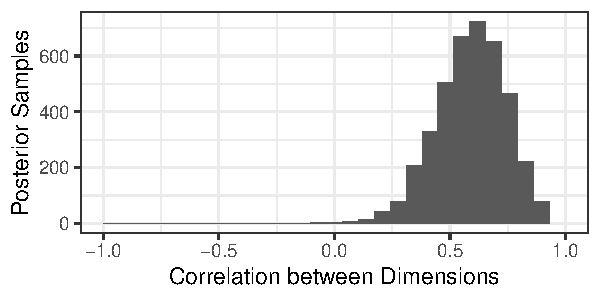
\includegraphics[width=0.45\textwidth]{../change/ornuhl-binom/categorical_order_gamma/fits/corr_sigma.pdf} &
		\\
		\textbf{(B)} & \textbf{(C)} \\
		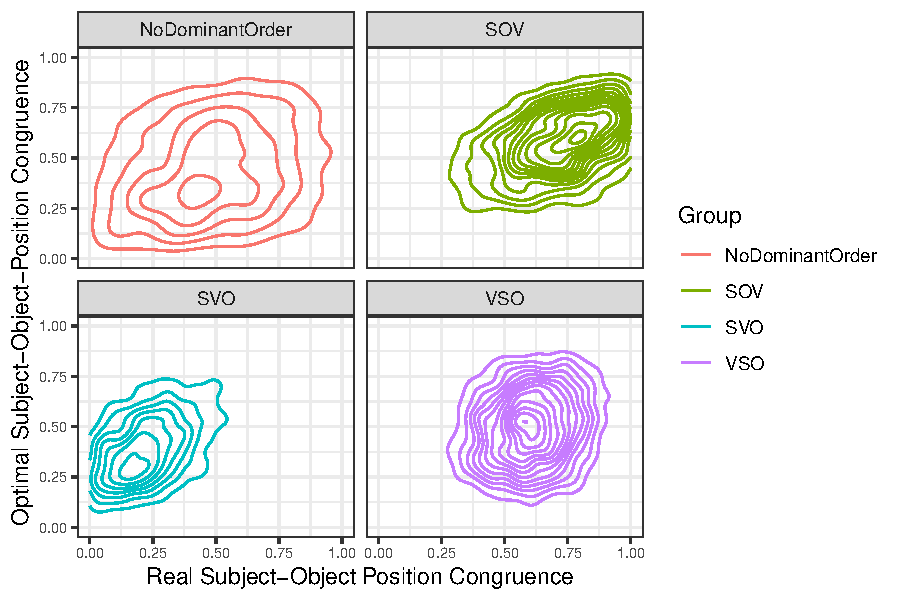
\includegraphics[width=0.5\textwidth]{../change/ornuhl-binom/categorical_order_gamma/fits/stationary_case_facet.pdf} &
    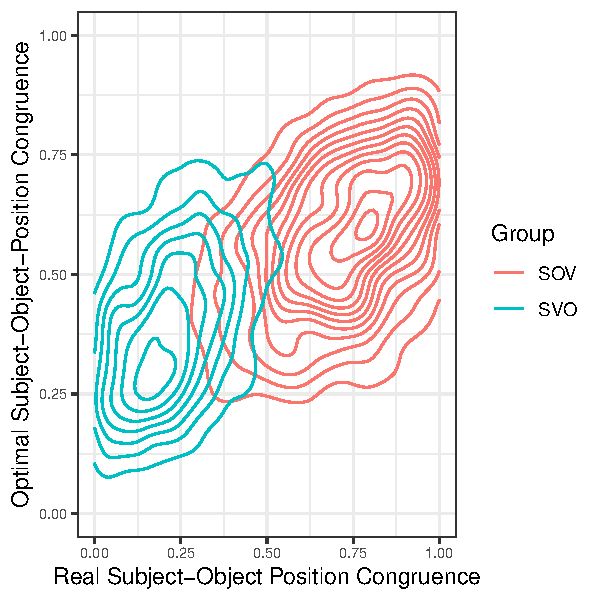
\includegraphics[width=0.4\textwidth]{../change/ornuhl-binom/categorical_order_gamma/fits/stationary_case_svo_sov.pdf}
	\end{tabular}
	\caption{Results of the phylogenetic analysis, controlling for conventional categorical word order labels. (A) Posterior over the correlation component $R_\Sigma$. Positive values indicate that grammar and usage evolve together. (B) Estimated stationary distributions for the four word order categories. (C) Estimated stationary distributions for the frequent classes, SOV and SVO.}
    \label{fig:langs-categorical}
\end{figure}


\paragraph{Results}
We show results in Figure~\ref{fig:langs-categorical}.
The posterior of $\Sigma$ (Figure~\ref{fig:langs-categorical} (A)) is very similar to the posterior in the main analysis; almost all of the posterior mass is on positive correlations between grammar and usage components ($R = 0.40$, 95\% credible interval [0.01, 0.71], $P(R<0) = 0.023$). % change/ornuhl-binom/case/separate_b/fits/correlation_sigma.txt
This shows that languages display coadaptation of grammar and usage even \emph{beyond} what is captured by conventional categorical word order labels.
Note that an association between grammar and usage on the level of categorical word order labels would already constitute evidence for coadaptation; this result shows that coadaptation happens at the more fine-grained level of subject-object position congruence.
In Figure~\ref{fig:langs-categorical} (B-C), we show the resulting stationary distributions for all four categorical word order types (B), and for the two frequent ones (SOV/SVO, (C)).
In the case of the frequent categories (SOV, SVO), the stationary distributions show a correlation in the two axes, illustrating that coadaptation happens even within these categorical classes.

\section{The Role of Case Marking}

Here, we test whether changes in the presence of case marking might mediate the coupling between word order and usage patterns.
We do this by fitting an extension of the model that can model different directions of change in languages with and without case marking, and checking whether the analysis continues to provide evidence for coevolution between word order and usage \emph{even beyond} what is captured by correlations of usage and word order with the presence of case marking.


\paragraph{Coding Languages for Case Marking}
We coded languages from our sample for the presence or absence of case marking on the basis of \citep{wals-49}, supplemented with information from the grammatical literature where no information was provided.
We amended the annotation from \citep{wals-49} to include only case marking that distinguishes between subjects and objects; this concerns several modern Celtic and Germanic languages, which have some nominal case marking but do not distinguish subjects and objects (e.g., Swedish and English use -\textit{s} to mark possessives, but do not distinguish nominal subjects and objects.).

We furthermore coded all interior nodes of the phylogenetic tree for case marking based on the linguistic literature.
In some cases, this annotation was unambiguous due to available historical documentation even though no treebank data was available (e.g., Proto-West-Scandinavian was a late form of Old Norse and had case markers).
In many other cases, cognate case markers are unambiguously attested both within and without a group, showing that they were present in the protolanguage (e.g., Proto-Germanic, Proto-Indo-Iranian).
Furthermore, in many protolanguages, case markers are commonly reconstructed based on their presence in different descendant branches (e.g., Proto-Indo-European, Proto-Afroasiatic, Proto-Common-Turkic, Proto-Uralic and Proto-Ugric). % Uraloc: Abondolo Uralic; Hajdu uralischen Sprachen; Marcantonio Uralic
Case is not unambiguously reconstructed for Proto-Niger-Congo; we verified that both possible parameter settings lead to qualitatively equivalent results (we report results under the assumption that it did not have case, with essentially indistinguishable results for the other cases).

\paragraph{Model of Change conditioned on Case Marking}
Based on the prior literature, we expect that languages without case marking will be biased towards low subject-object position congruence~\citep{vennemann1974explanation}.
To take this into account, we modified the model by conditioning the mean vector $\mu$ on the presence or absence of case in the language $L$.
\begin{equation*}
    \operatorname{d}\xi_{L,t} = \Gamma_{C(L)} \cdot (\xi_{L,t}-\mu_{C(L)}) \operatorname{d}t + \Lambda \operatorname{d}B_t
\end{equation*}
where $C(L)$ is $1$ if $L$ has case and $0$ else.
We set priors $\mu_{C(L)} \sim N(0,1)$ for both $C(L) = 0$, and $1$.

\paragraph{Results}
We plot the distribution of languages and the fitted stationary distributions, conditioned on $C(L)$, in Figure~\ref{fig:langs-case} (B-C).
In accordance with the prior literature, the model indicated that languages without case marking favor regions with low observed and optimized subject-object position congruence.
For languages with case marking, there was evidence for a bias towards higher subject-object position congruence.
We plot the posterior of the correlation component of $\Sigma$ (see Section~\ref{sec:instant-corr}) in Figure~\ref{fig:langs-case} (A).
The posterior probability that the correlation is $\leq 0$ is estimated to be $0.023$.
This shows that languages show coadaptation beyond usage and grammar in basic word order, even beyond an association with case marking.

\paragraph{Conclusion}
We found that, while case marking has a robust impact on subject-object position congruence, coadaptation continues to hold when controlling for this.

\begin{figure}
    \centering
	\begin{tabular}{cccc}
		\textbf{(A)} \\
		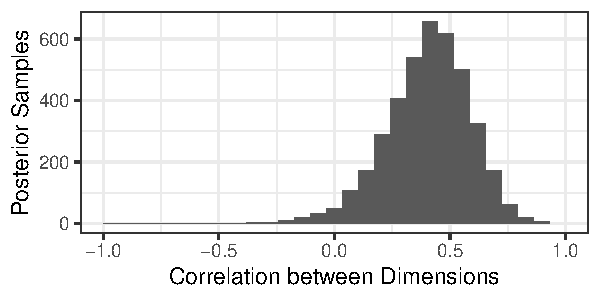
\includegraphics[width=0.5\textwidth]{../change/ornuhl-binom/case/separate_b/fits/corr_sigma.pdf} &
		\textbf{(B)} & \textbf{(C)} \\
		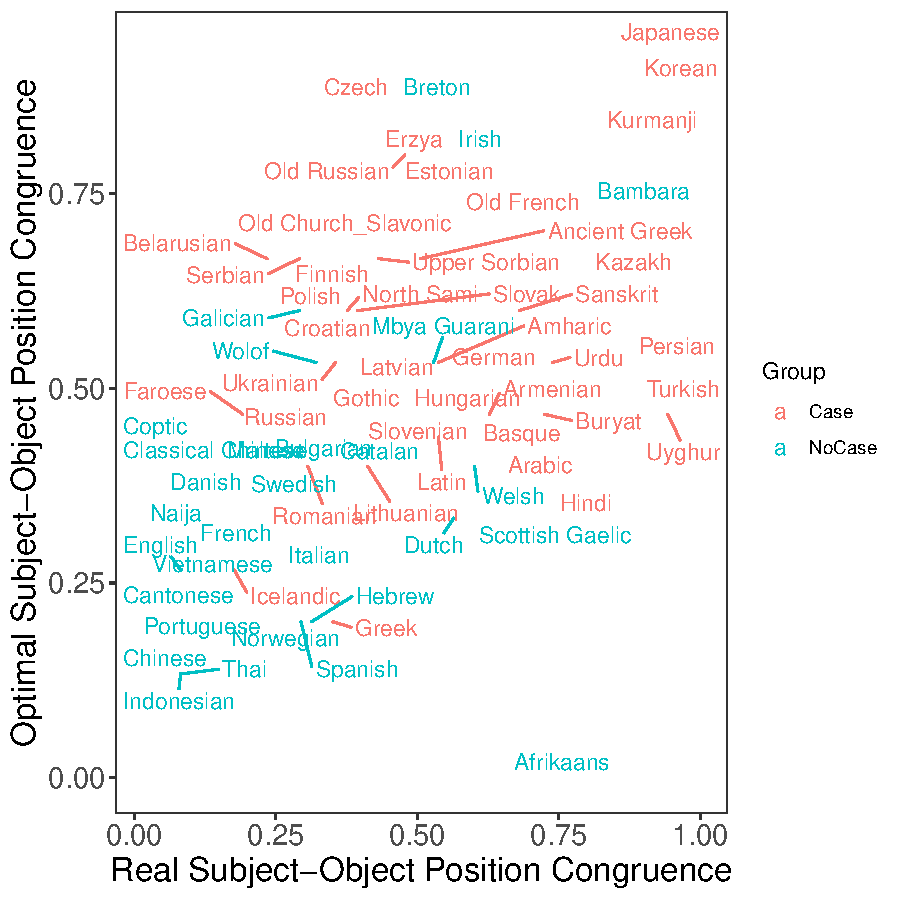
\includegraphics[width=0.5\textwidth]{../analysis/figures/by_patient_marking.pdf} &
    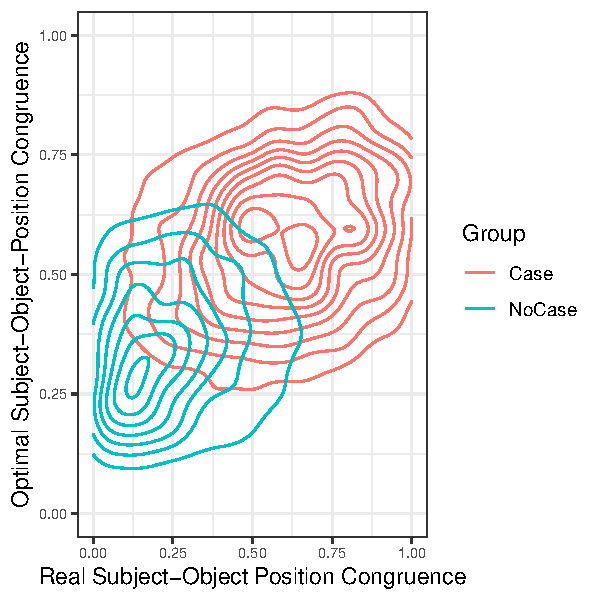
\includegraphics[width=0.5\textwidth]{../change/ornuhl-binom/case/separate_b/fits/stationary_case.pdf}
	\end{tabular}
    \caption{Posterior of the correlation component $R_\Sigma$ (see Section~\ref{sec:instant-corr}) when accounting for case marking. Left: Languages by availability of morphological distinction between subject and object nouns. Right: Fitted stationary distribution, conditioned on case marking.}
    \label{fig:langs-case}
\end{figure}

%#Oliver A. Iggesen. 2013. Number of Cases.
%#In: Dryer, Matthew S. & Haspelmath, Martin (eds.)
%#The World Atlas of Language Structures Online.
%#Leipzig: Max Planck Institute for Evolutionary Anthropology.
%#(Available online at http://wals.info/chapter/49, Accessed on 2020-09-20.)


%\section{Pro-Drop}
%This correlation was not accounted for by differences in the availability of pro-drop (see SI Section X).


%Say something specific:
%Furthermore, we specifically considered what distinguishes the tree topologies of Old English from those of Modern English.
%- Old English -- English what distinguishes the tree structures?
%In this respect, Old English patterned more like contemporary Japanese.


%\subsection{Pro Drop}

%\subsection{Subject-Verb Agreement}

\section{Within-Language Correlates of Basic Word Order}

Here, we show that basic word order reflects optimization for Dependency Length Minimization (DLM) not only on the level of languages, but also on the level of individual sentences.

%\subsection{Coexpression: VS Order in SVO Languages}
In many SVO languages, certain intransitive subjects can appear after the verb (``along came a dog'').
This kind of ``intransitive inversion'' has been documented in many SVO languages, including English, Romance languages, and Chinese \citep[Chapter 17.2]{li1981mandarin}.
There are also languages whose basic word order is different in transitive and in intransitive clauses \citep{wals-82}; the World Atlas of Language Structures lists 13 languages with transitive SVO and intransitive VS basic word order \citep{wals-81,wals-82}, while it lists no languages with transitive VSO and intransitive SV order.
This observation has been formalized as the following language universal: \textit{If VS is dominant with transitives, it is also dominant with intransitives} (\citet[No 344]{plank2000the}, citing \citet{kozinsky1981Nekotorye}).
DLM provides an explanation for this universal.

%- literature
%- Unaccusative inversion
%-- Leonetti, Two Types of postervbal subject (Spanish): Unaccusative inversion (p. 17)
%-- English there inversion

We conjectured that, more generally, the rate of VS order is higher when no object is present than when an object is present.
For each language in our dataset, we collected statistics for all verbs with a subject and conducted the following logistic analysis:

\begin{equation}
\text{SV Order} \sim \text{Object is present}
\end{equation}

A positive effect indicates that presence of an object makes SV order more likely, compared to VS order.
Results are shown in Table S16.
As predicted, in most languages where there is variation between SV and VS order, a significant positive effect was observed.

\begin{longtable}{l|lllllll}
	\multicolumn{4}{p{0.8\textwidth}}{Table S16: Coefficients in logistic analysis regressing SV/VS Order based on the presence of an object. `SV Frequency' indicates the overall rate of SV order (as opposed to VS) in the language. A positive coefficient ($\beta > 0$) indicates that SV is more common in the presence of an object than when there is no object.}
	\\
		\multicolumn{4}{p{0.8\textwidth}}{}\\
Language & SV Frequency & $\beta$ & $p$ \\ \hline
Afrikaans  &  0.9924497  &  -0.01379332  &  0.9650237 \\ 
Amharic  &  0.6643902  &  -0.3797678  &  0.001219969 \\ 
Ancient-Greek  &  0.7859838  &  0.3038916  &  1.848185e-24 \\ 
Arabic  &  0.4907006  &  0.5554177  &  1.267416e-64 \\ 
Armenian  &  0.8902104  &  0.8341103  &  1.601689e-07 \\ 
Bambara  &  0.9994276  &  16.98415  &  0.9967891 \\ 
Basque  &  0.8720129  &  -0.1103043  &  0.08111242 \\ 
Belarusian  &  0.7852564  &  2.020933  &  7.652911e-12 \\ 
Breton  &  0.5386905  &  0.06466503  &  0.7752487 \\ 
Bulgarian  &  0.8129963  &  1.286377  &  1.746863e-86 \\ 
Buryat  &  0.9964093  &  -0.4223533  &  0.7310379 \\ 
Cantonese  &  0.9936709  &  1.123673  &  0.3060742 \\ 
Catalan  &  0.9320653  &  0.06848983  &  0.05660422 \\ 
Chinese  &  0.9985795  &  17.70084  &  0.9849879 \\ 
Classical-Chinese  &  0.9992515  &  17.76376  &  0.9908623 \\ 
Coptic  &  0.9244142  &  5.31238  &  1.152644e-07 \\ 
Croatian  &  0.8270117  &  0.9824862  &  5.645664e-76 \\ 
Czech  &  0.7356542  &  0.4654191  &  8.203554e-233 \\ 
Danish  &  0.8646074  &  0.6166254  &  2.973047e-23 \\ 
Dutch  &  0.8128943  &  0.4173131  &  2.151784e-29 \\ 
English  &  0.9615841  &  3.441798  &  6.999747e-82 \\ 
Erzya  &  0.6735219  &  0.9077625  &  1.577672e-07 \\ 
Estonian  &  0.7320824  &  0.4946462  &  3.289869e-72 \\ 
Faroese  &  0.8431877  &  0.339571  &  0.3222813 \\ 
Finnish  &  0.8659807  &  1.249505  &  7.16487e-134 \\ 
French  &  0.957291  &  1.18344  &  5.68542e-114 \\ 
Galician  &  0.8767828  &  1.085919  &  1.407192e-57 \\ 
Gothic  &  0.7328141  &  0.6042657  &  2.057858e-12 \\ 
Greek  &  0.8386661  &  0.6462003  &  1.887567e-10 \\ 
Hebrew  &  0.6916882  &  0.926865  &  1.208581e-39 \\ 
Hindi  &  0.9959224  &  2.024877  &  1.667778e-09 \\ 
Hungarian  &  0.8099704  &  0.7695941  &  5.126524e-12 \\ 
Icelandic  &  0.8614551  &  0.2468021  &  0.09588306 \\ 
Indonesian  &  0.9785124  &  3.344637  &  2.340445e-13 \\ 
Irish  &  0.1545299  &  0.04717788  &  0.6933074 \\ 
Italian  &  0.820324  &  1.77427  &  0 \\ 
Japanese  &  1  &  -1.248811  &  0.9999989 \\ 
Kazakh  &  0.9917921  &  -0.3564089  &  0.6167294 \\ 
Korean  &  0.9999377  &  15.18245  &  0.9952635 \\ 
Kurmanji  &  0.9965278  &  16.56947  &  0.9948486 \\ 
Latin  &  0.8283322  &  0.5684388  &  2.631472e-36 \\ 
Latvian  &  0.7920269  &  0.7170238  &  1.130302e-48 \\ 
Lithuanian  &  0.7858136  &  0.2974647  &  0.002695024 \\ 
Maltese  &  0.7308357  &  2.338013  &  4.368465e-22 \\ 
Mbya-Guarani  &  0.8694158  &  1.774875  &  0.08476647 \\ 
Naija  &  0.9928428  &  17.72801  &  0.9752152 \\ 
North-Sami  &  0.7980562  &  1.91703  &  3.563754e-36 \\ 
Norwegian  &  0.8351502  &  0.8743093  &  2.509498e-273 \\ 
Old-Church-Slavonic  &  0.6860935  &  0.7588353  &  9.248082e-20 \\ 
Old-French  &  0.861299  &  0.7790791  &  5.314585e-66 \\ 
Old-Russian  &  0.6607248  &  0.3806921  &  2.224959e-15 \\ 
Persian  &  0.9957089  &  0.05733093  &  0.8792901 \\ 
Polish  &  0.7560659  &  0.8276517  &  7.551643e-111 \\ 
Portuguese  &  0.9085286  &  2.148836  &  1.403539e-207 \\ 
Romanian  &  0.7327803  &  0.5733261  &  3.711964e-91 \\ 
Russian  &  0.7753686  &  1.072127  &  0 \\ 
Sanskrit  &  0.8934502  &  0.3507692  &  0.009118983 \\ 
Scottish-Gaelic  &  0.0153741  &  -0.3860788  &  0.4179889 \\ 
Serbian  &  0.8013561  &  1.359499  &  2.642889e-58 \\ 
Slovak  &  0.7235023  &  0.7112696  &  4.069385e-30 \\ 
Slovenian  &  0.777516  &  0.3698094  &  4.000879e-11 \\ 
Spanish  &  0.8737669  &  0.7861673  &  4.765933e-186 \\ 
Swedish  &  0.8646589  &  0.7199364  &  2.120114e-58 \\ 
Thai  &  0.9992459  &  17.44808  &  0.9967014 \\ 
Turkish  &  0.9739342  &  -0.7741544  &  1.351646e-08 \\ 
Ukrainian  &  0.8057971  &  1.053127  &  6.439663e-48 \\ 
Urdu  &  0.996012  &  1.243488  &  0.003855179 \\ 
Uyghur  &  0.9605438  &  2.694296  &  4.241587e-06 \\ 
Vietnamese  &  0.9890523  &  0.76429  &  0.02094286 \\ 
Welsh  &  0.06223176  &  0.5705449  &  0.2071651 \\ 
Wolof  &  0.999068  &  16.69683  &  0.9914133 \\ 
Yoruba  &  0.9954023  &  1.140257  &  0.3086771 \\ 

\end{longtable}




%\subsection{Embedding: VSO in Embedded Clauses, SVO in Main Clauses}
In some predominant VSO languages, SVO is an alternative word order in unembedded clauses, whereas embedded clauses tend to only allow VSO.
This is in accordance with the predictions of DLM, which favors high subject-object position congruence in embedded clauses (see Figure 1B in the main paper).
Examples include relative clauses in Afroasiatic and Celtic (Standard Arabic~\citep{alqurashi:2012}, Breton \citep[][p. 80]{timm1988relative}, Ancient Egyptian \citep{gardiner1957egyptian}, Tuareg \citep[Chapter 12.1.2]{heath2005a}).
Conversely, in some SVO languages, embedded clauses show VSO order (Bantu, \citet{demuth1999verb}); Miza (Chadic) has SVO/VOS in main clauses and VOS in embedded clauses~\citep{wals-81}.
However, it is not generally true that VS order is more common in embedded clauses across all languages that have variation in basic word order.
For instance, German and Dutch can have VS in main clauses, but are almost always SV in subordinate clauses; the same holds for Quileute (Chimakuan)~\citep{wals-81}.




%\section{Detailed Diachronic Trajectories}
%-- coexpression
%-- position congruence
%-- case
%- English
%- French?
%- Ancient Greek?

\section{Estimating Usage and Grammar on Disjoint Corpora}


\begin{figure}
	\begin{center}
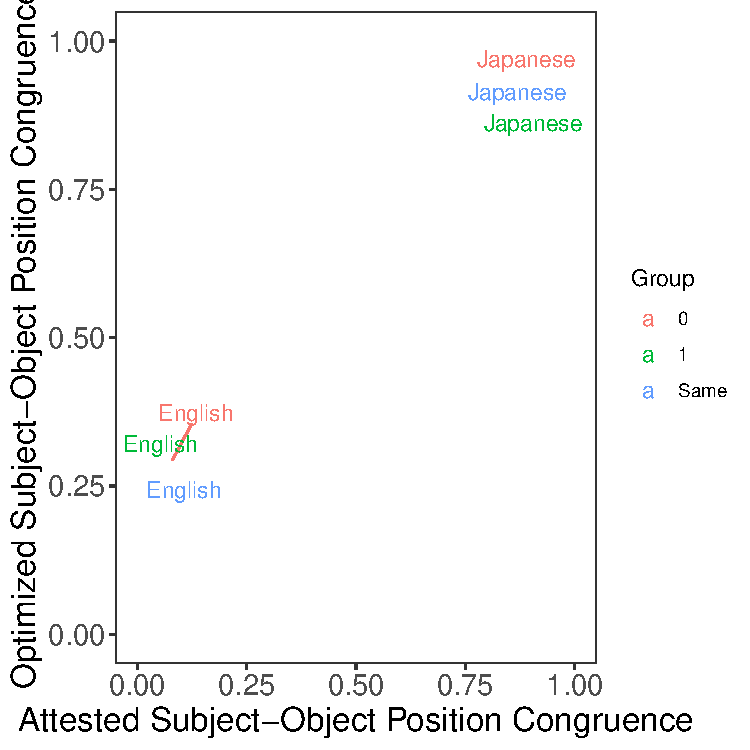
\includegraphics[width=0.6\textwidth]{../disjoint/plane-disjoint.pdf}
	\end{center}
	\caption{Estimating attested and optimized subject-object position congruence on disjoint datasets in English and Japanese. The blue datapoints are the results from the main experiments. For the other datapoints, we randomly split each of the corpora in half, and estimated attested and optimized position congruence separately on the two disjoint subsets.}\label{fig:disjoint}
\end{figure}

In the main experiment, we used the same corpora to estimate attested and optimized position congruence.
This is not circular, as optimized position congruence is estimated only on the basis of the tree topologies, without any influence from the actually observed orderings.
Here, we illustrate that equivalent results are obtained even when estimating both quantities on \emph{entirely disjoint} corpora.
Fot this, we randomly split the English and Japanese data into two equal-sized parts A and B.
In Figure~\ref{fig:disjoint}, we report the results obtained by (1) estimating optimized congruence on A and attested congruence on B (red), (2) the same with A and B reversed (blue), (3) and for comparison the result from the main experiment, where both quantities are estimated on the full dataset, i.e., the union of A and B.
The results show that qualitatively equivalent results are obtained in all three cases.

%\mhahn{TODO. Here, my plan is to illustrate that estimating quantities on disjoint corpora makes no difference, using just two or three languages as examples.}



\section{Coexpression of Subjects and Objects}
In Figure~\ref{fig:study2}, we show attested subject-object congruence together with the fraction of verbs that simultaneously express a subject and an object, for each language.
As described in the main paper, in a linear mixed-effects model, with by-family intercept and slope, attested subject-object position congruence was predictive of this fraction ($\beta=-0.09$, $SE=0.05$, $95\%$ credible interval $[-0.19, 0.0]$, $\operatorname{P}(\beta<0) = 0.029$). % analysis/coexpression/coexpression_results.txt 


\begin{figure}
    \centering
    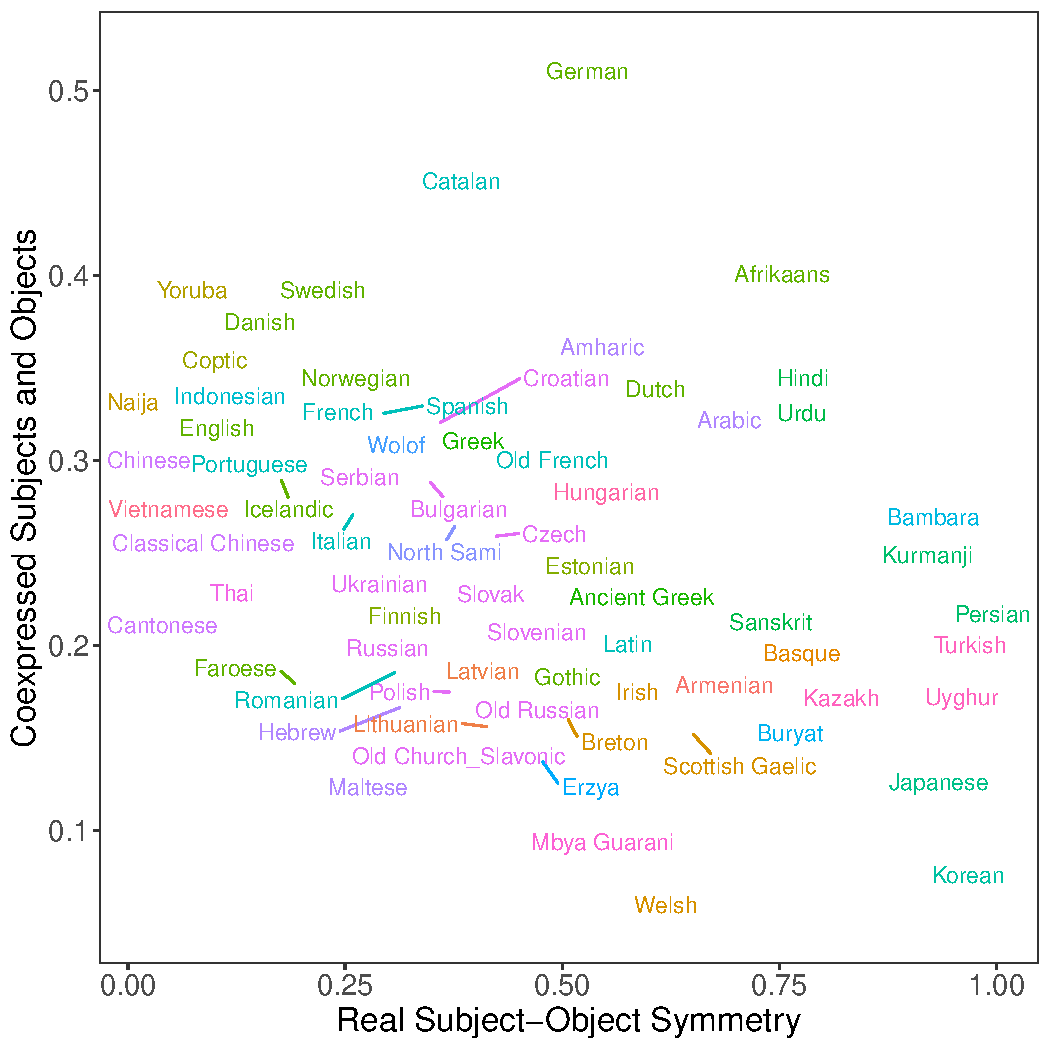
\includegraphics[width=0.7\textwidth]{../analysis/figures/objects-order-pureud-byVerb_FORMAT.pdf}
    \caption{Comparison of attested subject-object position congruence (x-axis) and the fraction of verbs that simultaneously express a subject and an object (y-axis).}
    \label{fig:study2}
\end{figure}


\section{Details for Mixed-Effects Analyses}

\paragraph{Priors}

We conducted standard Bayesian linear mixed-effects regressions \citep{gelman1995bayesian} where the response $y_i$ belonging to language $i$ is given by
\begin{equation}
	y_i = (\alpha + \alpha_{p_i}) + (\beta + \beta_{p_i}) x_i + \epsilon_i
\end{equation}
where $x_i$ is the predictor (e.g., attested subject-object position congruence), $p_i$ is the phylum of language $i$, $\epsilon_i \sim \mathcal{N}(0,\sigma^2)$, and $\alpha_{p_i}$ and $\beta_{p_i}$ are per-phylum adjustments to the intercept $\alpha$ and the slope $\beta$ respectively.

As described in the main paper, following \citep{burkner2018advanced}, we assumed a uniform prior for the fixed effect slopes and the intercepts, and a weakly informative prior (Student's $t$ with $\nu=3$ degrees of freedom, location 0, and scale $\sigma=2.5$) for the variance components, and an LKJ(1) prior \citep{lewandowski2009generating} for the covariance matrix of random effects. 


%\paragraph{Detailed Results}

%for position congruence:
%
%- logistic
%
%- linear
%
%Frequentist: 
%- Coefficients
%
%- R2
%
%Bayesian: Bayesian
%
%- Coefficients: ...
%
%- R2: $0.46$, 95\% CrI $[0.28, 0.59]$.
%
%for coexpression:

%
%                       Estimate Est.Error l-95% CI u-95% CI Rhat Bulk_ESS
%Intercept                  0.48      0.04     0.40     0.56 1.00     1742
%OSSameSide_Real_Prob.C     0.41      0.12     0.18     0.66 1.00     2460


\paragraph{Frequentist Analyses}

We also conducted analogous frequentist analyses using lme4~\citep{bates-fitting-2015}.
%output/landscapes_2.6.R_brms_genera_linear_lme4.txt
When  predicting optimized subject-object position congruence from attested subject-object position congruence, the frequentist analysis yielded a slope of $0.44$ (SE $0.094$, $t=4.70$), with $R^2 = 0.28$.
When predicting coexpression of subjects and objects from attested subject-object position congruence, the slope was $\beta=-0.10$ (SE $0.039$, $t=-2.56$), with $R^2=0.10$.


%\begin{tabular}{lllll}
%	& $\beta$ & $SE$ & $t$ \\
%	Intercept & 0.29168 & 0.04254 & 6.856 \\
%	Attested S.O. Pos. Cong. & 0.44261 & 0.09424 & 4.697
%\end{tabular}


\paragraph{Insensitivity to Priors}

A potential concern is that, because our dataset includes many phyla represented by only one or a few languages, the mixed-effects model might suffer from inflated estimates of the variance components, as the slopes cannot be individually estimated for those phyla.

We repeated the analysis predicting optimized subject-object position congruence with several more strongly regularizing priors on both the variance components and the slope $\beta$.

In Figure~\ref{fig:variance-priors}, we plot how the posteriors for $\beta$, the variance $\tau^2$ of the per-phylum adjustments $\beta_p$, and the response variance $\sigma^2$ vary as a function of the prior.
Results show that, while more strongly regularizing priors shrink the estimated range of $\tau^2$, they have little impact on the posterior of the key quantity, $\beta$.


\begin{figure}
	\begin{tabular}{c||ccccc}
		Prior & $\beta$ & Variance $\tau^2$ of Random Slope & Response Variance $\sigma^2$ \\  \hline\hline
$\sigma^2, \tau^2 \sim t(3,0,2.5)$ &
	\multirow{3}{*}{	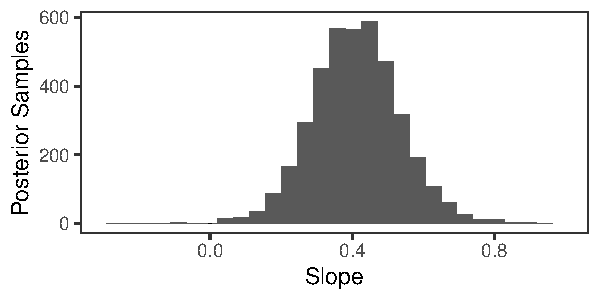
\includegraphics[width=0.25\textwidth]{../analysis/posteriors-across-priors/student_3_0_25_uniform-beta.pdf}} &
	\multirow{3}{*}{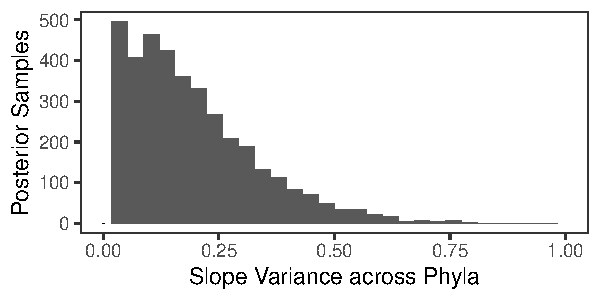
\includegraphics[width=0.25\textwidth]{../analysis/posteriors-across-priors/student_3_0_25_uniform-across-phyla-variance.pdf}} &
	\multirow{3}{*}{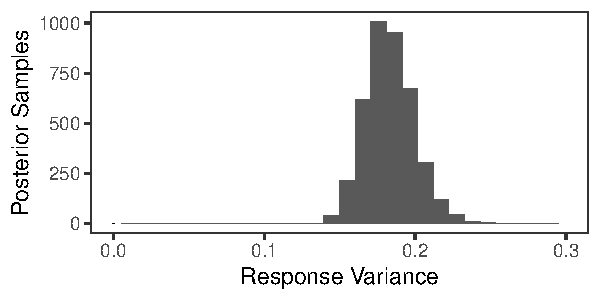
\includegraphics[width=0.25\textwidth]{../analysis/posteriors-across-priors/student_3_0_25_uniform-response-variance.pdf} }
\\
		$\beta \sim Unif$ \\
		$\alpha \sim t(3,0.5,2.5)$ \\
\\ \hline\hline
		$\sigma^2, \tau^2, \beta \sim t(3,0,2.5)$ &
{	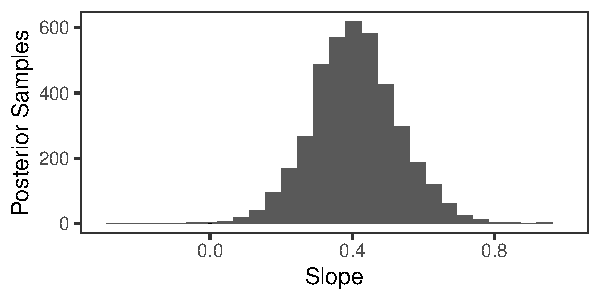
\includegraphics[width=0.25\textwidth]{../analysis/posteriors-across-priors/student_3_0_25-beta.pdf}} &
{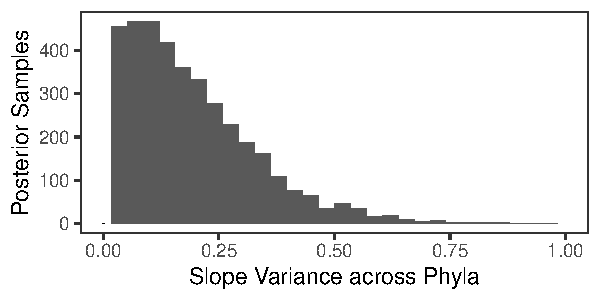
\includegraphics[width=0.25\textwidth]{../analysis/posteriors-across-priors/student_3_0_25-across-phyla-variance.pdf}} &
{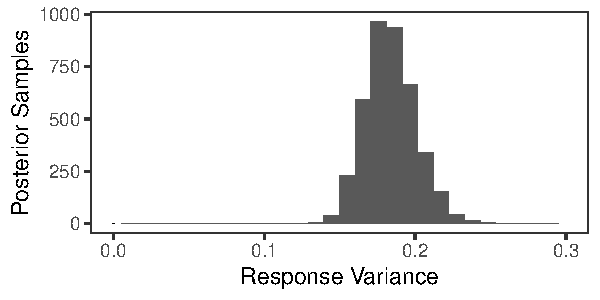
\includegraphics[width=0.25\textwidth]{../analysis/posteriors-across-priors/student_3_0_25-response-variance.pdf} }
\\ \hline
			$\sigma^2, \tau^2, \beta \sim t(3,0,10)$ &
		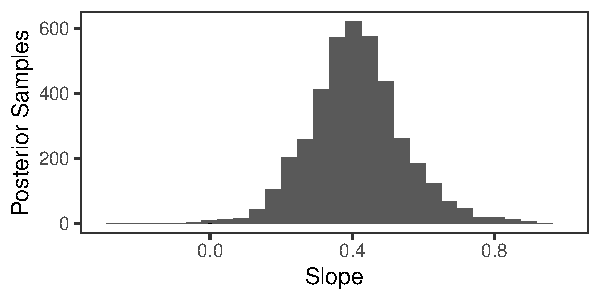
\includegraphics[width=0.25\textwidth]{../analysis/posteriors-across-priors/student_3_0_10-beta.pdf} &
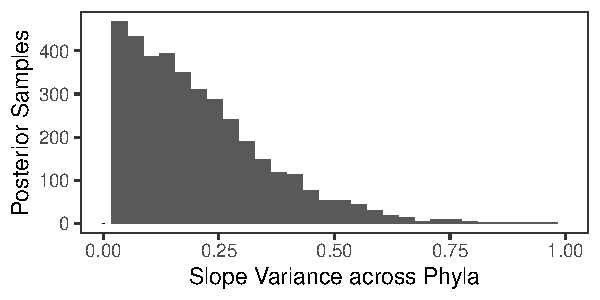
\includegraphics[width=0.25\textwidth]{../analysis/posteriors-across-priors/student_3_0_10-across-phyla-variance.pdf} &
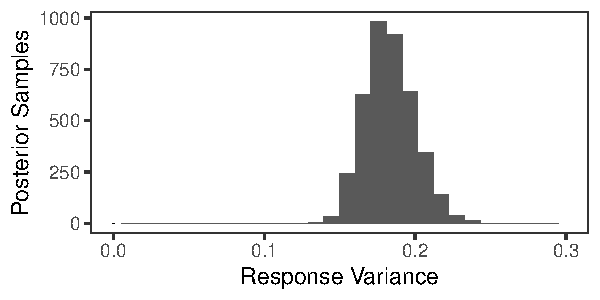
\includegraphics[width=0.25\textwidth]{../analysis/posteriors-across-priors/student_3_0_10-response-variance.pdf} 
\\ \hline
		$\sigma^2, \tau^2, \beta \sim \mathcal{N}(0,1)$ &
		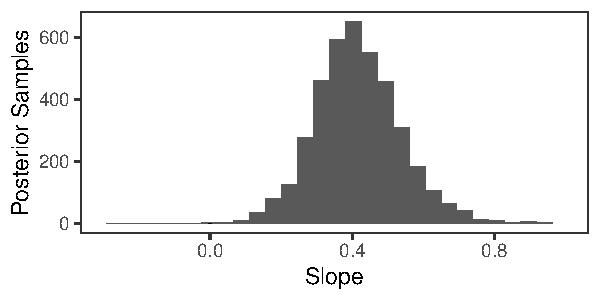
\includegraphics[width=0.25\textwidth]{../analysis/posteriors-across-priors/normal_0_1-beta.pdf} &
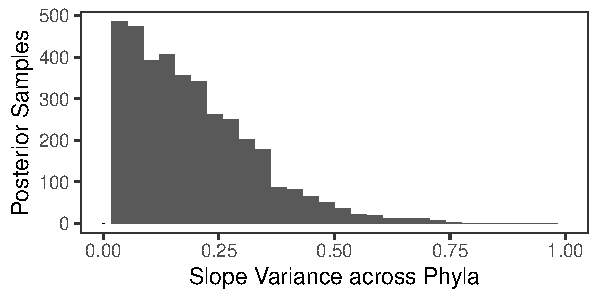
\includegraphics[width=0.25\textwidth]{../analysis/posteriors-across-priors/normal_0_1-across-phyla-variance.pdf} &
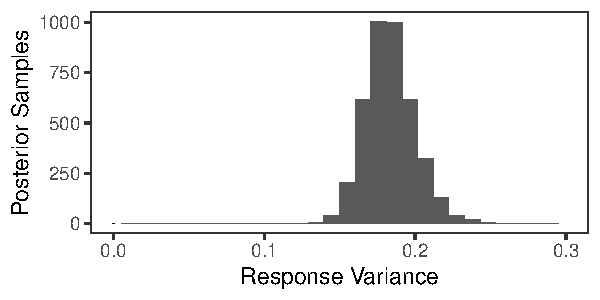
\includegraphics[width=0.25\textwidth]{../analysis/posteriors-across-priors/normal_0_1-response-variance.pdf} 
\\ \hline
$\sigma^2, \tau^2, \beta \sim t(3,0,0.5)$ &
		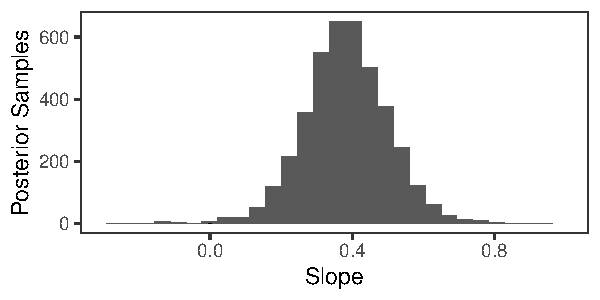
\includegraphics[width=0.25\textwidth]{../analysis/posteriors-across-priors/student_3_0_05-beta.pdf} &
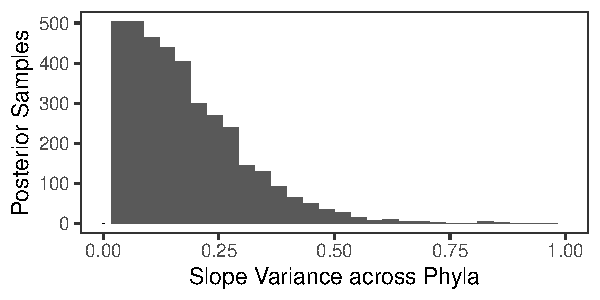
\includegraphics[width=0.25\textwidth]{../analysis/posteriors-across-priors/student_3_0_05-across-phyla-variance.pdf} &
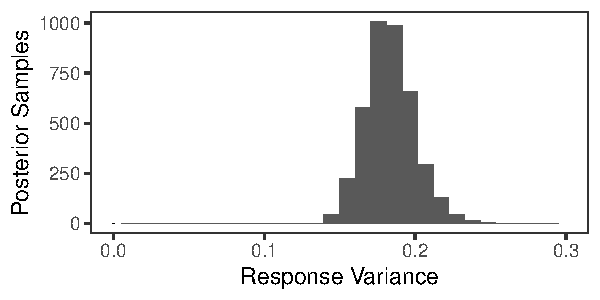
\includegraphics[width=0.25\textwidth]{../analysis/posteriors-across-priors/student_3_0_05-response-variance.pdf} 
\\ \hline
		$\sigma^2, \tau^2, \beta \sim t(3,0,0.1)$ &
		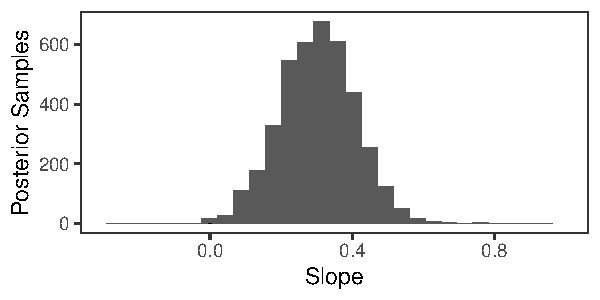
\includegraphics[width=0.25\textwidth]{../analysis/posteriors-across-priors/student_3_0_01-beta.pdf} &
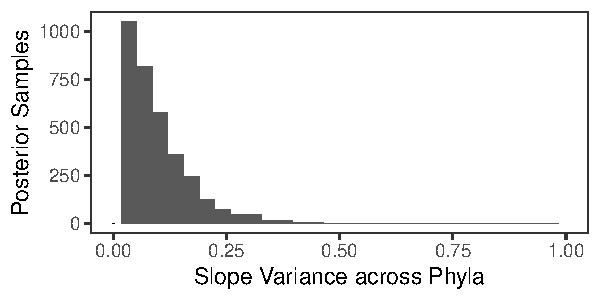
\includegraphics[width=0.25\textwidth]{../analysis/posteriors-across-priors/student_3_0_01-across-phyla-variance.pdf} &
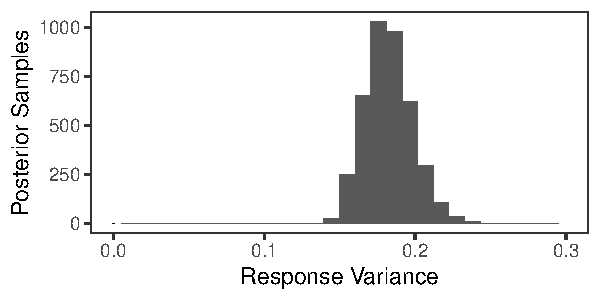
\includegraphics[width=0.25\textwidth]{../analysis/posteriors-across-priors/student_3_0_01-response-variance.pdf} 
\\ \hline
	\end{tabular}
	\caption{Impact on the prior for the variance terms on the posterior in the Bayesian mixed-effects analysis.
	The first line corresponds to the prior used in our analysis; the other priors differ in the degree to which they regularize towards $0$, from little regularization (top) to very strong regularization (bottom).
	For each prior, we show the posterior of the coefficient $\beta$ (the quantity of interest), the variance of the slope across phyla, and the variance of the Gaussian response. While changing the prior affects the estimated posterior of the slope variance across phyla, it has little effect on the estimate of $\beta$.}\label{fig:variance-priors}
\end{figure}






%
%\section{Analyses Excluding Indo-European}
%
%Available corpus data strongly overrepresent the Indo-European language family.
%Here, we show that the results of our analyses do not depend on the presence of this particular family.
%
%
%%
%%\begin{figure}
%%    \centering
%%    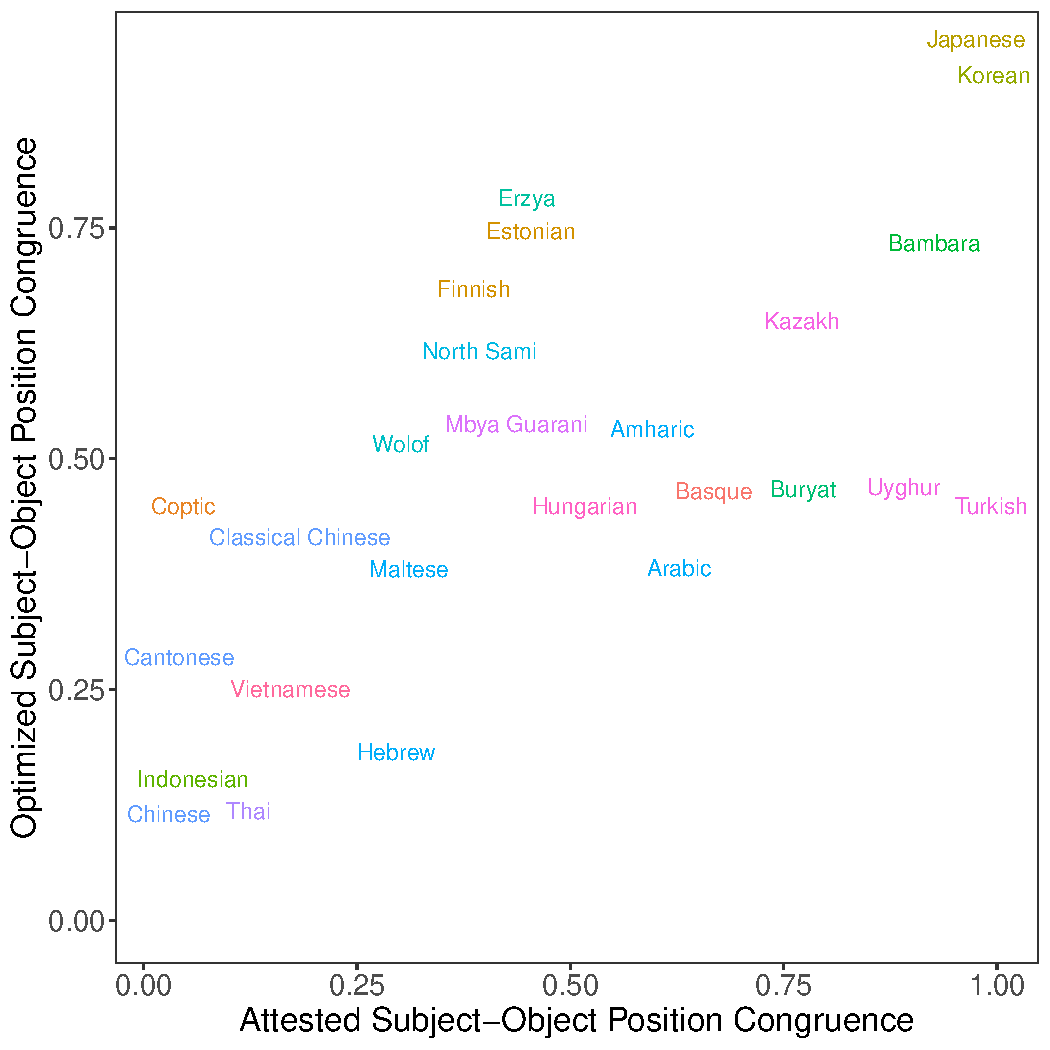
\includegraphics[width=0.7\textwidth]{../analysis/figures/fracion-optimized_DLM_2.6_format_NoIE.pdf}
%%    \caption{Attested and optimized subject-object position congruence of non-Indo-European languages.}
%%    \label{fig:todo}
%%\end{figure}
%%
%%
%
%
%\paragraph{Correlation}
%
%Excluding Indo-European, the Pearson correlation between optimized and attested subject-object position congruence is $R=0.68$, $95\%$ CI $[0.40, 0.85]$, $p = 0.00013$.
%
%
%
%\paragraph{Mixed-Effects Analysis Excluding Indo-European}
%
%Excluding Indo-European, the coefficient is $\beta=0.80$, $SE=0.32$, $95\%$ CrI $[0.17, 1.47]$.
%


%\paragraph{Phylogenetic Analysis Excluding Indo-European}
%We next fitted the phylogenetic model excluding all Indo-European languages.
%
%- posterior. compare parameters to the setting without
%
%The parameter of interest is the stationary correlation between usage and grammar components.
%
%- Bayes Factor compared to model without correlation

%\section{Further Statistical Analyses}
%TODO
%
\paragraph{Per-Phylum Results and Fitted Slopes}


\begin{figure*}
    \centering
            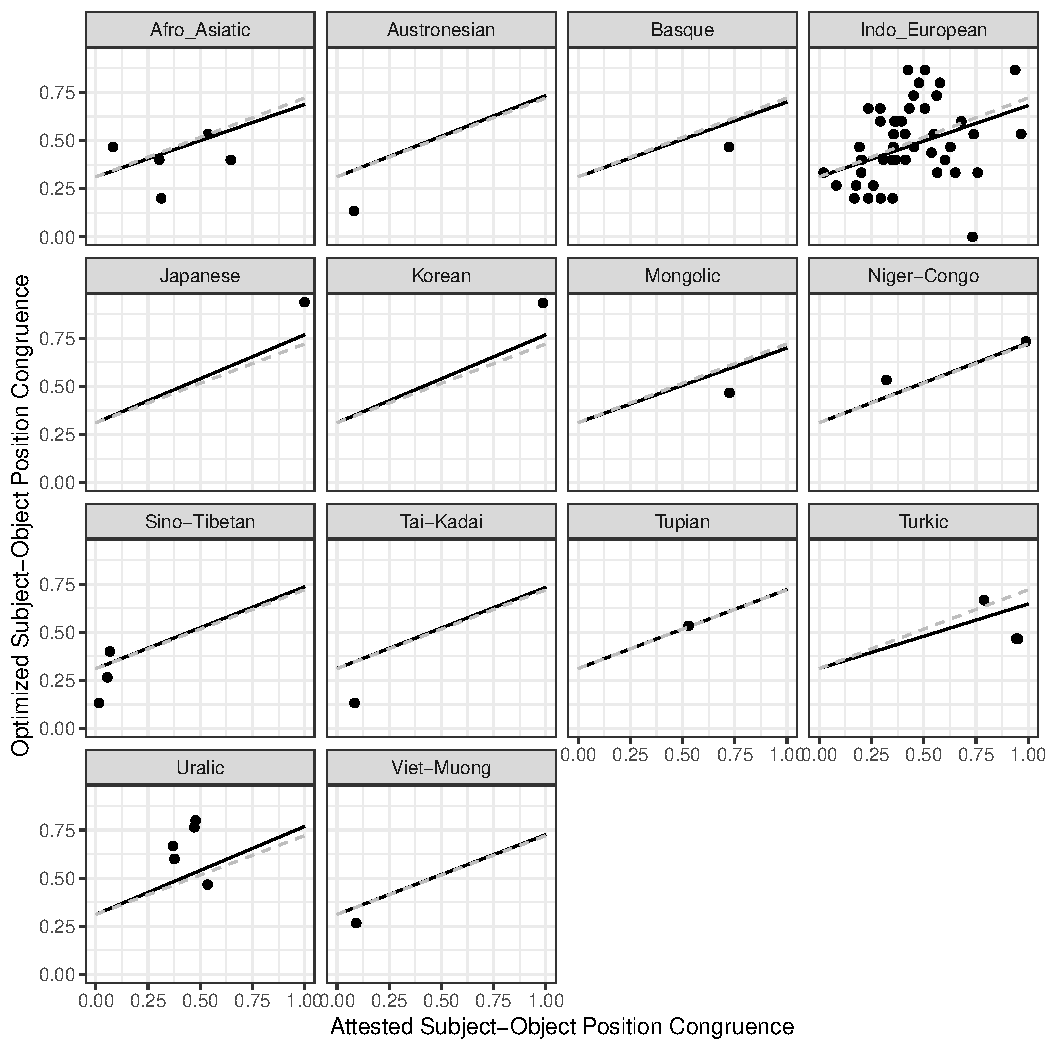
\includegraphics[width=0.4\textwidth]{../analysis/figures-scratch/byPhylum_all_slopes.pdf}
%
                 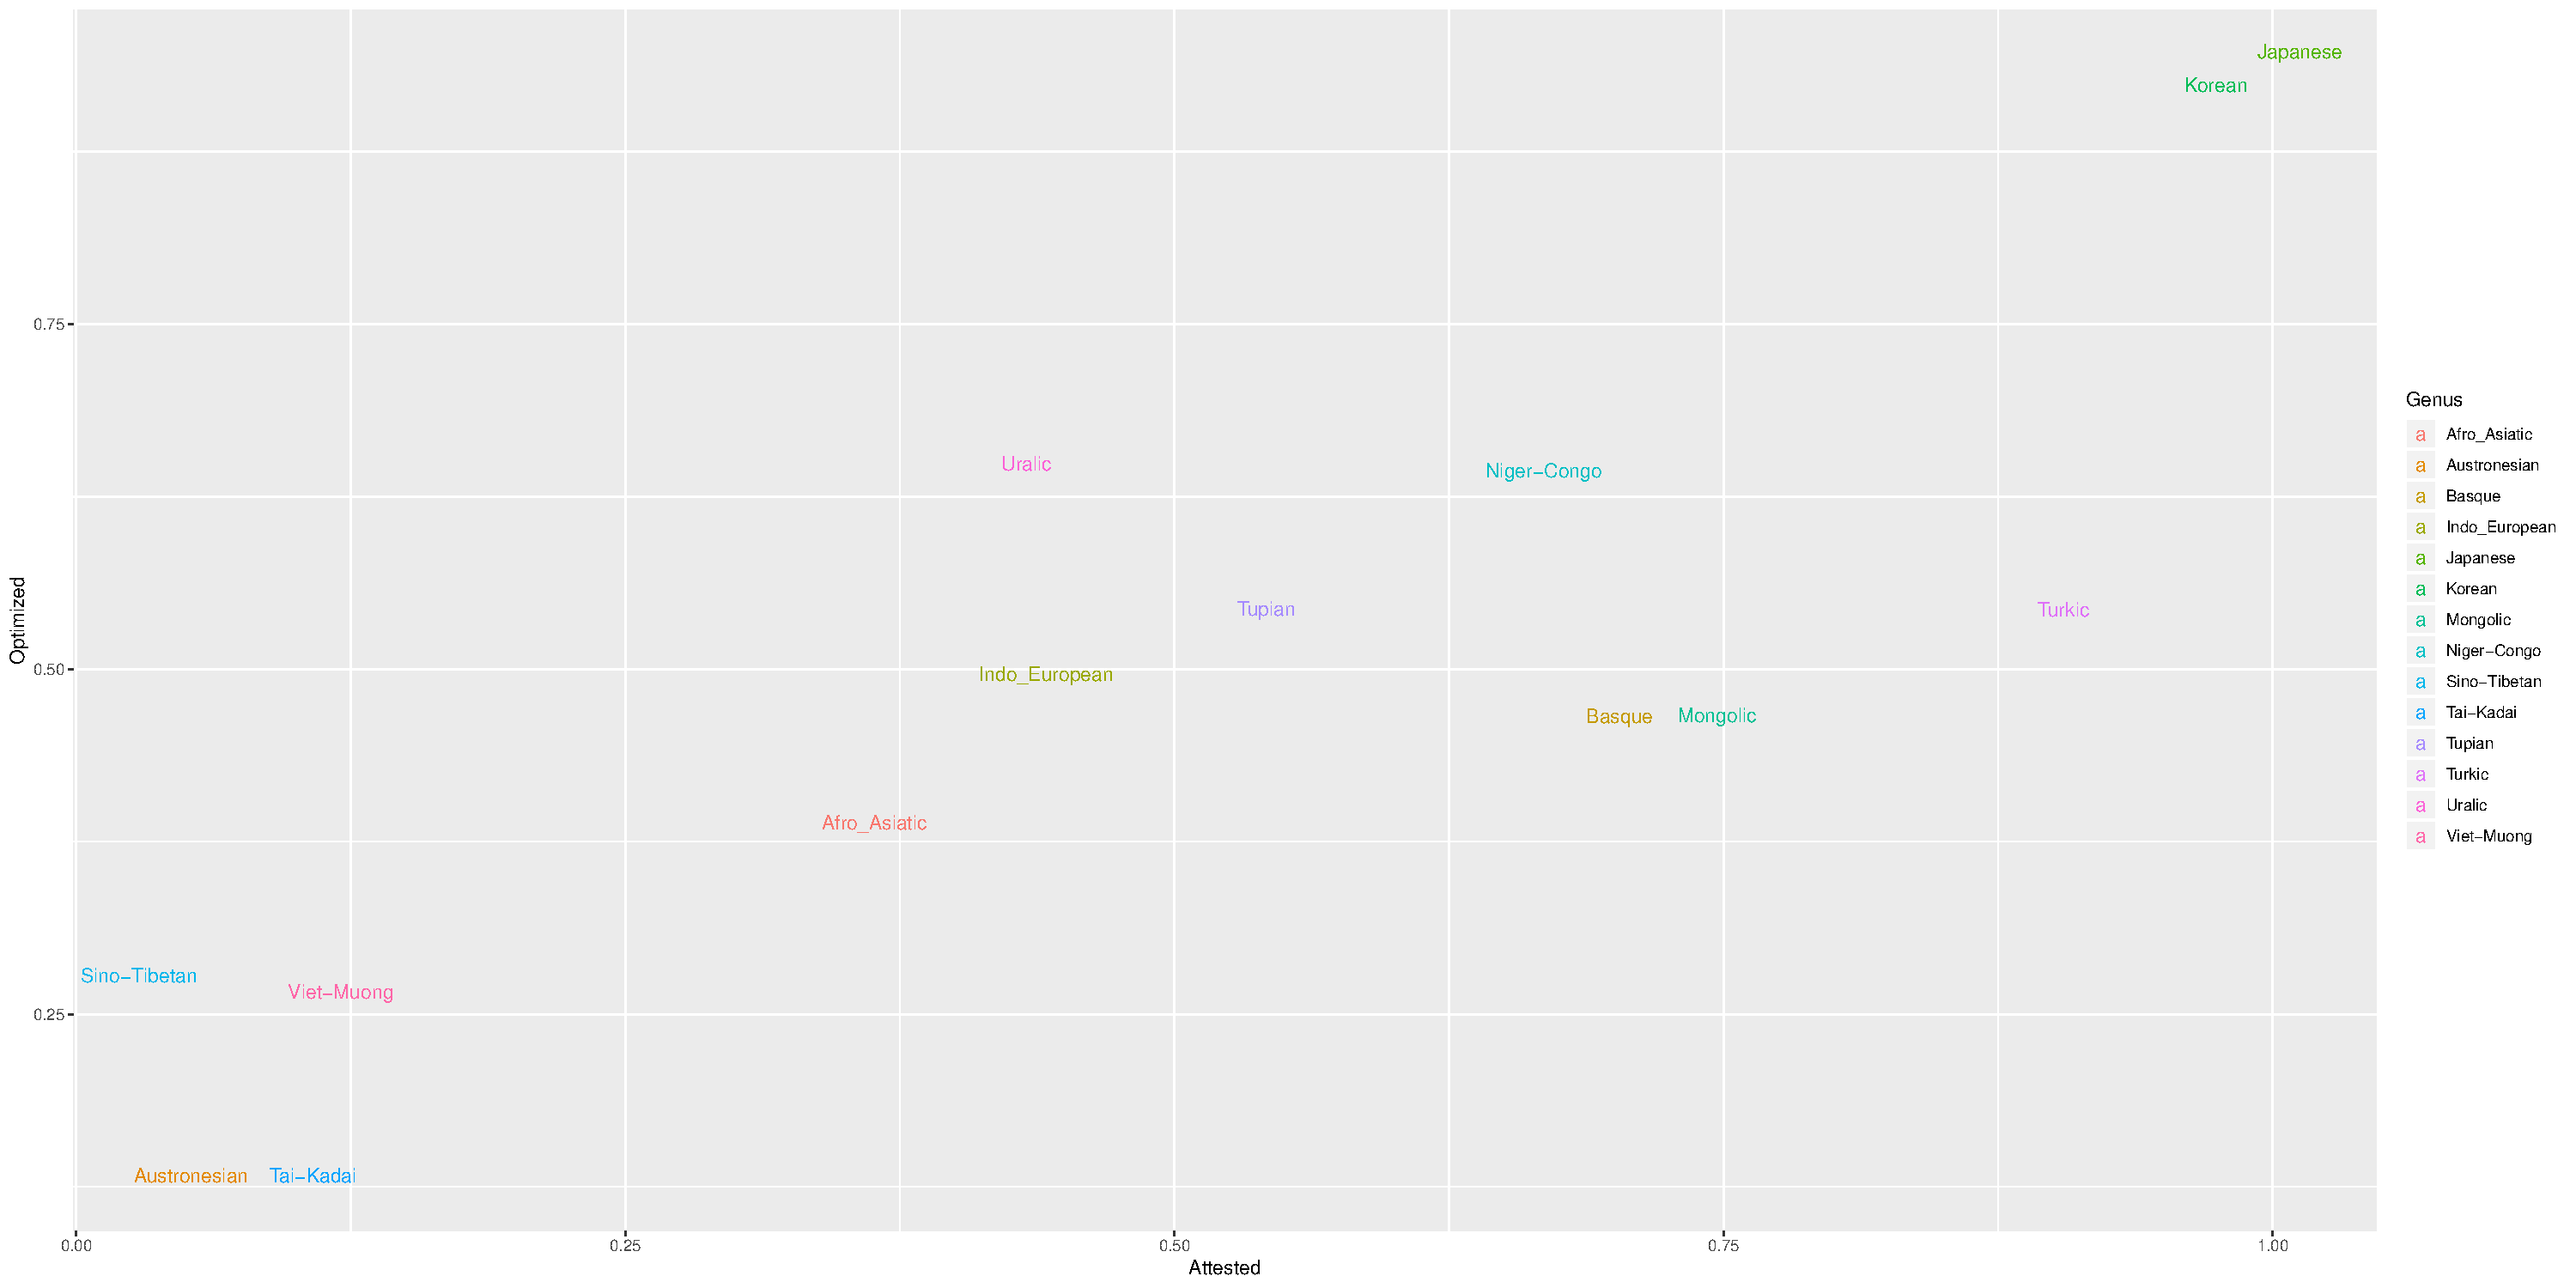
\includegraphics[width=0.4\textwidth]{../analysis/figures-scratch/per-phylum-means.pdf}

    \caption{Left: Fit of the mixed-effects model across the 14 phyla. We show the overall slope as a dashed line, and the per-phylum adjusted slope as a solid line. Right: Mean attested and optimized subject-object position congruences per phylum.}
    \label{fig:per-phylum-plot}
\end{figure*}

Figure~\ref{fig:per-phylum-plot} shows results across the 14 phyla for the analysis of optimized and attested subject-object position congruence.

Note that most individual phyla do not provide sufficient evidence for a linear relationship on their own.
However, for the mixed-effects model, estimating the overall slope does not require independent estimates of the slopes in each phylum.
Instead, the mixed-effects regression obtains its slope estimate by combining (i) the data across isolates and smaller phyla, and (ii)the slope within the well-represented Indo-European phylum.

In Figure~\ref{fig:per-phylum-posteriors-1}, we show the fitted slope $\beta+\beta_p$ for each phylum that has at least two languages.
Across phyla, the model fits a very similar slope.


\begin{figure*}
    \centering
            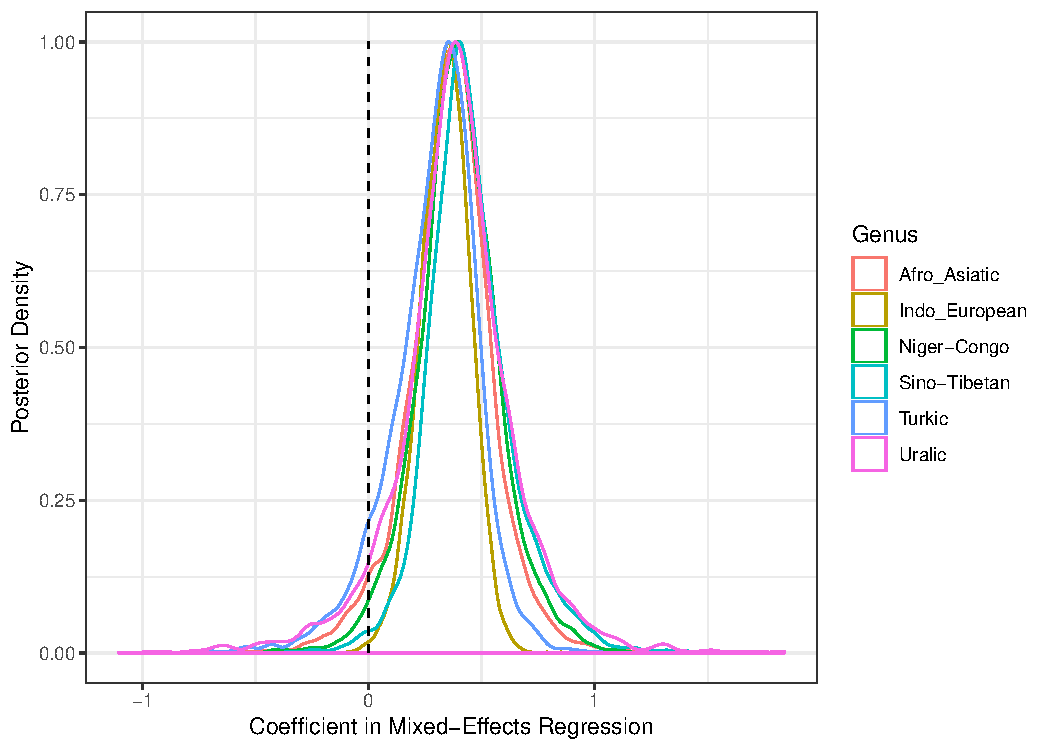
\includegraphics[width=0.8\textwidth]{../analysis/figures-scratch/per-phylum-posteriors.pdf}
     \caption{Posterior Densities for the slope in the linear mixed-effects regression in the six phyla with at least two languages. Across phyla, the model fits a very similar slope.}
    \label{fig:per-phylum-posteriors-1}
\end{figure*}



\begin{figure*}
    \centering
            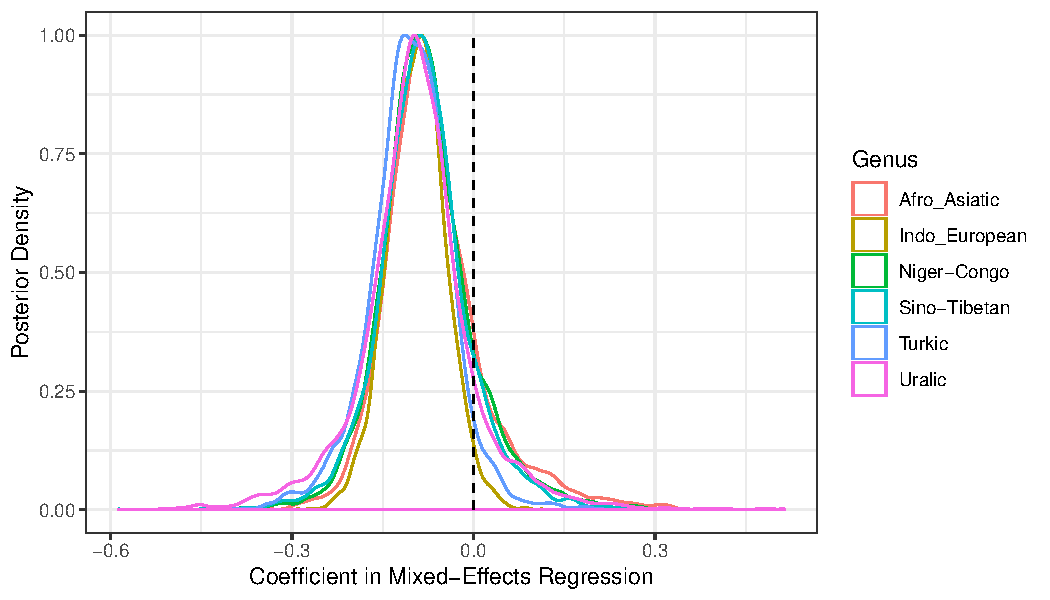
\includegraphics[width=0.8\textwidth]{../analysis/figures-scratch/coexpression-per-phylum-posteriors.pdf}
     \caption{Posterior Densities for the slope in the linear mixed-effects regression in the six phyla with at least two languages. Across phyla, the model fits a very similar slope.}
    \label{fig:per-phylum-posteriors-2}
\end{figure*}





\section{Sensitivity to Corpus Size}

Here, we provide evidence that estimates of attested and optimized subject-object position congruence are stable across corpus sizes.
For English and Japanese, we estimated attested and optimized subject-object position congruence on randomly sampled subsets of 500, 1000, 5000, 10000 sentences.
Results are shown in Figure~\ref{fig:congruence-by-size}, together with figures for the full corpora (31,811 sentences in English; 67,002 sentences in Japanese).
The results show that, while there is some variation across corpus sizes, estimates are quite stable even when comparing the full corpus to a subset of only 500 sentences.


\begin{figure}
    \centering
    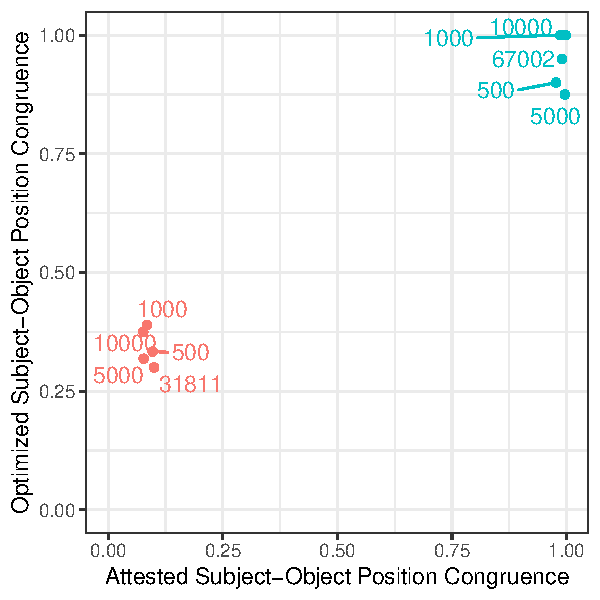
\includegraphics[width=0.7\textwidth]{../analysis/subset/figures/by-corpus-size.pdf}
    \caption{Attested and optimized subject-object position congruence as a function of the number of sentences included in the corpus.}
    \label{fig:congruence-by-size}
\end{figure}


\section{Causality}

Here, we show that available corpus data is compatible with different possible causal directions between usage and grammar.
Recall the model of change described in the main paper:
\begin{equation*}
    \operatorname{d}\xi_{L,t} = \Gamma \cdot (\xi_{L,t}-\mu) \operatorname{d}t + \Lambda \operatorname{d}B_t
\end{equation*}
where $\mu \in \mathbb{R}^2$,  $\Gamma, \Lambda \in \mathbb{R}^{2\times 2}$ are non-degenerate matrices, $\Gamma$ is diagonal with positive entries, and $B_t$ is Brownian motion in two dimensions.

This model describes how change tends to be correlated in usage and grammar, and does not encode a direction of causal effect between usage and grammar.
This model is derived from the standard Independent Contrasts model of coevolving traits~\citep{felsenstein1973maximum,freckleton2012fast}.
It formalizes a process of coevolution where usage and grammar evolve in tandem, without one asymmetrically influecing the other.

However, one can also construct Ornstein-Uhlenbeck processes that explicitly encode asymmetric influence between the two traits by considering cases where the matrix $\Gamma$ is not symmetric \citep{ait-sahalia2008closed, https://doi.org/10.1111/biom.13292}.
Based on this idea, we considered a model in which one dimenion (e.g., $\xi_1$) changes independently, whereas the other one (e.g., $\xi_2$) changes in response to the first one:
\begin{align*}
	\operatorname{d}(\xi_1)_{L,t} &= \Gamma_{11} \cdot ((\xi_1)_{L,t}-\mu_1) \operatorname{d}t + \Lambda_{11} \operatorname{d}B_t \\
	\operatorname{d}(\xi_2)_{L,t} &= \Gamma_{22} \cdot ((\xi_2)_{L,t}-\mu_2) \operatorname{d}t + \Gamma_{12} \cdot ((\xi_1)_{L,t}-\mu_1) \operatorname{d}t + \Lambda_{22} \operatorname{d}B_t \\
\end{align*}
This model arises from the previous one by making $\Lambda$ diagonal and allowing $\Gamma_{12} \neq 0$.
The key component is the blue term, which expresses an asymmetric influence of $\xi_1$ on changes in $\xi_2$.
The strength and direction of influence of $\xi_1$ on $\xi_2$ is expressed by the coefficient $\Gamma_{12}$.
We placed a prior $\Gamma_{12} \sim \mathcal{N}(0,1)$.

An analogous model is obtained in which $\xi_2$ causes changes in $\xi_1$.
In total, we compared three models: the coevolution model from the main paper, an asymmetric model where grammar shapes usage, and an asymmetric model where usage shapes grammar.
%The three models can be distinguished in principle, but this may require high temporal resolution in data.


We compared marginal likelihood across the three models in Table~\ref{tab:causal}, together with the lesioned model without any correlation between usage and grammar, as described in the main paper.
On our dataset, all three models provide almost the same marginal likelihood, improving by approximately the same amount over the lesioned model.
This shows that currently available data does not make it possible to decide whether there is a single asymmetric causal direction between usage and grammar across languages.


\begin{table}
	\begin{center}
\begin{tabular}{l|llll}
	Model & Marginal Log-Likelihood \\ \hline\hline
	Coevolution (as described in Main Paper) & -32 \\
	Grammar shapes Usage & -32 \\
	Usage shapes Grammar & -32 \\ \hline
	Lesioned (no correlation, as described in Main Paper) & -38 \\
\end{tabular}
	\end{center}
	\caption{Comparing model fit for the coevolution model assumed in the main paper, and two explicitly causal models. All models assuming coevolution or an explicit causal direction achieve very similar model fit.}\label{tab:causal}
\end{table}


\section{Details on Ordering Grammars}

%\paragraph{Ordering Grammar Formalism}
We adopt the word order grammar formalism of \cite{gildea-optimizing-2007,gildea-grammars-2010,gildea-human-2015} to Universal Dependencies.
The original grammar formlism of \cite{gildea-optimizing-2007} is defined for constituency treebanks; it defines weights for each combination of parent and child constituent category (e.g., ``NP$\rightarrow$JJ'' for the position of the adjective within the noun phrase).
We adapt this to Universal Dependencies by defining weights for combinations of dependency relation labels, the part-of-speech label of the head, and the part-of-speech label of the dependent.

Dependents of a head are ordered in ascending order by their weights, so that dependents with negative weights appear before the head and dependents with positive weights appear after the head.

For instance, a grammar might define the weights (among others)
\begin{center}
    VERB $\xrightarrow{nsubj}$ NOUN : -0.8
    
    VERB $\xrightarrow{obj}$ NOUN : 0.3
\end{center}
Applying this to a simple transitive sentence would result in SVO order:

\begin{center}
\begin{dependency}[theme = simple]
   \begin{deptext}[column sep=1em]
          dogs \& bite \& people  \\
          NOUN \& VERB \& NOUN \\
   \end{deptext}
   \depedge{2}{1}{subj}
   \depedge{2}{3}{obj}
\end{dependency}
\end{center}
In contrast, the following grammar, where both weights are negative, results in SOV order:
\begin{center}
    VERB $\xrightarrow{nsubj}$ NOUN : -0.8
    
    VERB $\xrightarrow{obj}$ NOUN : -0.3
\end{center}
as in the following example:

\begin{center}
\begin{dependency}[theme = simple]
   \begin{deptext}[column sep=1em]
          dogs \& people \& bite  \\
          NOUN \& NOUN \& VERB \\
   \end{deptext}
   \depedge{3}{1}{subj}
   \depedge{3}{2}{obj}
\end{dependency}
\end{center}

Optimized and attested subject-object position congruence were calculated for dependencies of the form VERB $\xrightarrow{nsubj}$ NOUN.

In order to efficiently optimize grammars for dependency length, we adopt the gradient-based optimization method of \cite{hahn2020universals}. 
This method considers a probabilistic extension of the grammar formalism where each grammar defines a distribution over possible linearizations of a tree; grammars as defined above correspond to the special case where the distribution is always concentrated on one linearization (i.e., it is deterministic).
We refer to \cite{hahn2020universals} for the precise definition of this extension.
This extension makes the average dependency length a \emph{differentiable} function of the grammar parameters, opening the door to the use of gradient-based optimization algorithms for ordering grammars.
The optimization method then applies stochastic gradient descent using the REINFORCE estimator~\citep{williams-simple-1992} to optimize the average dependency length across the trees in the corpus and the possible linearizations of each tree.
Over the course of optimization, the probabilistic grammars converge to essentially deterministic ones that minimize average dependency length across the trees in the corpus.




\bibliography{literature}
\bibliographystyle{natbib}



\end{document}



\paragraph{Computing the Likelihood for Model with Changing Parameters}


\begin{equation}
\xi_{L,t'} | \xi_{L,t} \sim N\left(\mu' + e^{-\Delta \Gamma} (\xi_{L,t}-\mu'),\ \Omega - e^{-\Delta \Gamma} \Omega e^{-\Delta \Gamma^T}\right)
\end{equation}

Assume evolves according to $''$ parameters from $t'$ to $t''$ over time $\Delta''$.

\begin{align*}
\mathbb{E}[\xi_{L,t''} | \xi_{L,t}] &= \mathbb{E}\left[ \mathbb{E}[\xi_{L,t''} | \xi_{L,t'}] | \xi_{L,t}\right ] \\
&=  \mathbb{E}\left[  \mu'' + e^{-\Delta'' \Gamma''} (\xi_{L,t'}-\mu'')      | \xi_{L,t}\right ] \\
&= \mathbb{E}\left[  \mu'' | \xi_{L,t}\right ]  + \mathbb{E}\left[e^{-\Delta'' \Gamma''} (\xi_{L,t'}-\mu'')      | \xi_{L,t}\right ] \\
&= \mathbb{E}\left[  \mu'' | \xi_{L,t}\right ]  + e^{-\Delta'' \Gamma''} (\mathbb{E}\left[\xi_{L,t'}|\xi_{L,t}\right ]-\mu'')        \\
&= \mu'' + e^{-\Delta'' \Gamma''} ( \mu' + e^{-\Delta' \Gamma'} (\xi_{L,t}-\mu')    -\mu'') \\
&= \mu'' + e^{-\Delta'' \Gamma''} \mu' + e^{-\Delta'' \Gamma''} e^{-\Delta' \Gamma'} (\xi_{L,t}-\mu')    - e^{-\Delta'' \Gamma''} \mu'' \\
&= \mu'' + e^{-\Delta'' \Gamma''} \mu' + e^{-\Delta'' \Gamma''} e^{-\Delta' \Gamma'} \xi_{L,t}- e^{-\Delta'' \Gamma''} e^{-\Delta' \Gamma'}  \mu'    - e^{-\Delta'' \Gamma''} \mu'' \\
&= (1-e^{-\Delta'' \Gamma''}) \mu'' + e^{-\Delta'' \Gamma''} (1-e^{-\Delta' \Gamma'} ) \mu' + e^{-\Delta'' \Gamma''} e^{-\Delta' \Gamma'} \xi_{L,t}
\end{align*}

More generally:
\begin{align*}
    \mathbb{E}[\xi_{L,t_{K}} | \xi_{L,t_{0}}] = e^{-\Delta_K\Gamma_K} \dots e^{-\Delta_1\Gamma_1} \xi_{L,t_{0}} + \sum_{i=1}^K e^{-\Delta_K\Gamma_K} \dots e^{-\Delta_{i+1}\Gamma_{i+1}} (1-e^{-\Delta_{i}\Gamma_{i}}) \mu_i
\end{align*}


The cross-variance: Let $\xi_A$ be the last common ancestor.
\begin{align*}
    Cov(\xi_{1}, \xi_2) &= \mathbb{E}[ \mathbb{E}[\xi_1 \xi_2^T | \xi_A]] - \mathbb{E}[\xi_1] \mathbb{E}[\xi_1]^T \\
    &= \mathbb{E}[ \mathbb{E}[\xi_1| \xi_A] \mathbb{E}[\xi_2^T | \xi_A]] - \mathbb{E}[\xi_1] \mathbb{E}[\xi_1]^T  \\
    &= ... Var(\xi_A) ...
\end{align*}

The covariance, assuming this has developed from a draw $\xi_0$ from one of the stationary parts:
\begin{align*}
    \mathbb{E}[\xi_K \xi_K^T | \xi_0] &= \mathbb{E}\left[ \mathbb{E}[\xi_K \xi_K^T| \xi_{K-1}] | \xi_0\right] \\
    &=\mathbb{E}\left[  \Omega_K - e^{-\Delta_K \Gamma_K} \Omega_K e^{-\Delta_K \Gamma_K^T}  +  \mathbb{E}[\xi_K| \xi_{K-1}] \mathbb{E}[\xi_K^T| \xi_{K-1}]      | \xi_0\right] \\
    &=  \Omega_K - e^{-\Delta_K \Gamma_K} \Omega_K e^{-\Delta_K \Gamma_K^T}  +  \mathbb{E}\left[\mathbb{E}[\xi_K| \xi_{K-1}] \mathbb{E}[\xi_K^T| \xi_{K-1}]      | \xi_0\right] \\
    &=  \Omega_K - e^{-\Delta_K \Gamma_K} \Omega_K e^{-\Delta_K \Gamma_K^T}  +  \mathbb{E}\left[\mathbb{E}[\xi_K| \xi_{K-1}] \mathbb{E}[\xi_K^T| \xi_{K-1}]      | \xi_0\right] \\
    &=  \Omega_K - e^{-\Delta_K \Gamma_K} \Omega_K e^{-\Delta_K \Gamma_K^T}  + (1-e^{-\Delta_K \Gamma_K})\mu_K \mu_K^T (1-e^{-\Delta_K \Gamma_K})^T + e^{-\Delta_K\Gamma_K} \mathbb{E}\left[\xi_{K-1} \xi_{K-1}^T| \xi_0\right] e^{-\Delta_K\Gamma_K} \\
\end{align*}

So we have the recursive equation
\begin{equation}
V_K = \Omega_K - e^{-\Delta_K \Gamma_K} \Omega_K e^{-\Delta_K \Gamma_K^T}  + (1-e^{-\Delta_K \Gamma_K})\mu_K \mu_K^T (1-e^{-\Delta_K \Gamma_K})^T + e^{-\Delta_K\Gamma_K} V_{K-1} e^{-\Delta_K\Gamma_K}
\end{equation}
and 
\begin{align*}
\mathbb{E}[\xi_K \xi_K^T | \xi_0] & =  \sum_{i=1}^K e^{-\Delta_K\Gamma_K}\dots e^{-\Delta_{i+1}\Gamma_{i+1}} \Omega_K e^{-\Delta_{i+1}\Gamma_{i+1}}\dots e^{-\Delta_K\Gamma_K} \\
& - \sum_{i=1}^K e^{-\Delta_K\Gamma_K}\dots e^{-\Delta_{i}\Gamma_{i}} \Omega_K e^{-\Delta_{i}\Gamma_{i}}\dots e^{-\Delta_K\Gamma_K} \\
&+ \sum_{i=1}^K e^{-\Delta_K\Gamma_K}\dots e^{-\Delta_{i+1}\Gamma_{i+1}} (1-e^{-\Delta_i \Gamma_Ki})\mu_i \mu_i^T (1-e^{-\Delta_i \Gamma_i})^T e^{-\Delta_{i+1}\Gamma_{i+1}}\dots e^{-\Delta_K\Gamma_K} \\
\end{align*}






\begin{table}
\begin{tabular}{lllll}
Model & SDE & File & Log-Likelihood & loo \\ \hline
Uncorrelated   & $d\xi_t = \left(\begin{matrix} \sigma_1 & 0 \\ 0 & \sigma_2\end{matrix}\right) dW_t$ & 30.stan & -239\\
Correlated  & $d\xi_t = \left(\begin{matrix} \sigma_1 & \rho_1 \\ \rho_2 & \sigma_2\end{matrix}\right) dW_t$ & 27, 28, 29 & -197, -220, -195 \\
\hline
Correlated Drift & $d\xi_t = - \left(\begin{matrix} \gamma_1 & \gamma_{1,2} \\ \gamma_{2,1} & \gamma_{2,2}\end{matrix}\right) \left(\xi_t-\mu\right) dt + \left(\begin{matrix} \sigma_1 & 0 \\ 0 & \sigma_2\end{matrix}\right) dW_t$ & 28.stan & -297\\
Correlated + Drift & $d\xi_t = - \left(\begin{matrix} \gamma_1 & 0 \\ 0 & \gamma_{2,2}\end{matrix}\right) \left(\xi_t-\mu\right) dt + \left(\begin{matrix} \sigma_1 & \rho_1 \\ \rho_2 & \sigma_2\end{matrix}\right) dW_t$ & 26.stan & -303 \\
Uncorrelated + Drift & $d\xi_t = - \left(\begin{matrix} \gamma_1 & 0 \\ 0 & \gamma_{2,2}\end{matrix}\right) \left(\xi_t-\mu\right) dt + \left(\begin{matrix} \sigma_1 & 0 \\ 0 & \sigma_2\end{matrix}\right) dW_t$ & 25.stan & -343 \\
Correlated Drift & $d\xi_t = - \left(\begin{matrix} \gamma_1 & \gamma_{1,2} \\ \gamma_{2,1} & \gamma_{2,2}\end{matrix}\right) \left(\xi_t-\mu\right) dt + \left(\begin{matrix} \sigma_1 & \rho_1 \\ \rho_2 & \sigma_2\end{matrix}\right) dW_t$ & 27.stan & -297\\
\hline
Correlated  + Areas & $d\xi_t = - \left(\begin{matrix} \gamma_1 & 0 \\ 0 & \gamma_2\end{matrix}\right) \left(\xi_t-\mu(x)\right) dt + \left(\begin{matrix} \sigma_1 & \rho_1 \\ \rho_2 & \sigma_2\end{matrix}\right) dW_t$ & 29, 31, 32, 33 & -61, -69\\
Uncorrelated  + Areas & $d\xi_t = - \left(\begin{matrix} \gamma_1 & 0 \\ 0 & \gamma_2\end{matrix}\right) \left(\xi_t-\mu(x)\right) dt + \left(\begin{matrix} \sigma_1 & 0 \\ 0 & \sigma_2\end{matrix}\right) dW_t$ & 30 & 113\\
\hline
Correlated  + Area(t) & $d\xi_t = - \left(\begin{matrix} \gamma_1 & 0 \\ 0 & \gamma_2\end{matrix}\right) \left(\xi_t-\mu(x)\right) dt + \left(\begin{matrix} \sigma_1 & \rho_1 \\ \rho_2 & \sigma_2\end{matrix}\right) dW_t$ & 35, 36, 38 & -47, -72, -54\\
Uncorrelated  + Area(t) & $d\xi_t = - \left(\begin{matrix} \gamma_1 & 0 \\ 0 & \gamma_2\end{matrix}\right) \left(\xi_t-\mu(x)\right) dt + \left(\begin{matrix} \sigma_1 & 0 \\ 0 & \sigma_2\end{matrix}\right) dW_t$ & 37 & -109\\
\hline
\end{tabular}
\caption{Phylogenetic drift models. For each model, we provide a representation as a stochastic differential equation, and the logarithm of the estimated marginal likelihood.}
\end{table}

\begin{table}[]
    \centering
    \begin{tabular}{c|c}
   Parameter & Prior \\ 
  $\left(\begin{matrix} \sigma_1 & 0 \\ 0 & \sigma_2\end{matrix}\right)$       &  \\
         $\left(\begin{matrix} \sigma_1 & \rho_1 \\ \rho_2 & \sigma_2\end{matrix}\right)$ & 
    \end{tabular}
    \caption{Caption}
    \label{tab:my_label}
\end{table}
